\documentclass[a4paper,11pt,twoside,openright]{report}

\setlength{\parindent}{0pt}
\setlength{\parskip}{6pt plus 2pt minus 1pt}
\usepackage[latin1]{inputenc}
\usepackage[english]{babel}

\usepackage{graphicx}
\usepackage{subfigure}
\usepackage{lscape}
\usepackage{subfigure}
\usepackage{multirow}
\usepackage{color}
%\usepackage{epsfig}

\usepackage{listings}


\usepackage{amsmath}
\usepackage{amsfonts}
\usepackage{amssymb}
\usepackage[latin1]{inputenc}

\usepackage[pdftex,plainpages = false, pdf pagelabels,pdfpagelayout = useoutlines,bookmarks,bookmarksopen = true,bookmarksnumbered = true,breaklinks =true,linktocpage,pagebackref,colorlinks = true,linkcolor = black,urlcolor  = black, citecolor = black, anchorcolor =black,hyperindex=true, hyperfigures]{hyperref}

\usepackage{geometry}
\geometry{outer=35mm,inner=45mm,tmargin=35mm,bmargin=40mm}

%opening
\title{Electricity micro-markets in distribution power systems with distributed energy resources}
\author{Pol Olivella-Rosell}

\usepackage[intoc,prefix]{nomencl}

\usepackage{ifthen}
\makenomenclature

\begin{document}
\pagestyle{empty}

\begin{center}
{\Large \sc Universitat Polit\`{e}cnica de Catalunya} \vskip 5cm

{\Large \bf Electricity micro-markets in distribution power systems with distributed energy resources}

\vskip 2cm {PhD-candidate: Pol Olivella-Rosell} 
\vskip 0.5 cm {Advisors: Roberto Villaf\'{a}fila Robles $\&$ Andreas Sumper}
\vskip 4cm 
{PhD on Electrical Engineering} \vskip 0.5 cm {Escola T\`{e}cnica Superior d'Enginyeria Industrial de Barcelona} \vskip 0.5cm {\sc } {Thesis proposal} \vskip 0.5cm {June 2015}
\end{center}

\tableofcontents
\newpage

\pagestyle{plain}

\chapter*{Summary}
\label{cap:summary}
This thesis deals with the integration of distributed energy resources in the electricity market to contribute in the objective of reducing greenhouse gasses emissions. Moreover, the context of this thesis is the development of smart grid technologies to integrate more renewable generators in the system. 

Nowadays, the power system is evolving from centralized to distributed. There are different factors which provoke this change: distributed energy resources (DER) expansion, ICT technologies enabling the installation of sensors in the distribution grid, and the cost reduction of technologies like batteries, power electronics and photovoltaic panels. All these factors provoke that the flow in the power system can be bidirectional: transmission to distribution or vice versa.

The problem is to integrate large quantities of DER in the system. The obstacles are grid capacity, which has physical limitations, and costs and variability of renewable energies. The solution implemented in many countries like Spain, Germany and Denmark, to promote installation of renewable generators has been to subsidize the generators, and the grid operation and reinforcement. This option is not cost effective and the operation cost increases with the expansion of this model. Furthermore, renewable generators have no operation cost, hence they offer large amount of energy at price zero. Considering that the electricity markets are based on auctions at marginal price, if all the energy is offered at price zero, the price of electricity is zero. In this situation renewable generator owners do not receive any economic compensations for their energy and this represents an inefficiency of the system.  

This thesis proposes to create local electricity micro-markets at distribution level to manage the resources locally. Thanks to this, the current problems at distribution level due to the renewable generation could be solved locally with the management of electric vehicles, storage units and demand side management programs.

This micro-market could be divided in two sub-markets; before and after the wholesale day-ahead market.
The micro-market before the day-ahead market could permit to organize the resources one day before the consumption. Moreover, this market could permit to decide how to participate in the day-ahead market; to consume or inject energy from/to the grid.
However, the micro-market after the day-ahead market could deal with technical adjustments and could permit to correct the forecasting errors with local resources when the local system expects deviations. Both markets could permit to solve problems from renewable generators locally.

This thesis proposes to design the architecture of this micro-market, to simulate the system and then to implement the system in a laboratory platform to validate the simulation results.

\chapter{Objectives}
\label{cap:objectives}
The main objective is to reduce greenhouse gasses emissions and climate change through distributed renewable generation. 
The advantages are clear: non-polluting sources which produce locally reducing the losses in the grid. 
The drawback is that this system is much more complicated to operate. The electricity flow in power systems will be bidirectional instead of centralized system with unidirectional flows.

The objectives of European Union before 2020 are in this direction and they pretend to reduce a 20$\%$ the greenhouse gasses emissions from 1990 levels. To supply 20$\%$ of energy from renewable sources \cite{Directiva_renovables} and to reduce 20$\%$ total energy consumption with energy efficiency improvements \cite{Directiva_eficiencia}. Therefore, the development of distributed generation is a key factor to reach these objectives.

But the massive integration of distributed generation faces technical and economic challenges in the system operation. 
Technical constraints are related to the grid capacity to transmit the energy, and also related to system operation because sources like wind and photovoltaic have lots of variability. 
Economic constraints are related to the electricity market and renewable technology costs.

According to the problem explained before, the main objective is to design the rules of local electricity micro-markets which enables to integrate significant quantities of renewable energy at price zero, particularly PV and wind. 

Furthermore, EVs and stationary storage units can participate in the local electricity micro-market with the capacity to consume and generate according to the price signals. 

\section{Partial objectives}
To achieve the main objective of this thesis there are partial objectives that have to be accomplished.

First of all, it is necessary to design the architecture of the market to define the use cases, the information exchanged and the components needed. The methodology proposed for this objective is the SGAM one. 

The second partial objective is to create a battery model which enables the participation of stationary batteries in the local electricity micro-market.

After that, the architecture designed will be implemented in a simulation model to test all the use cases of the market. The simulation model will include DER like PV and wind generators, EVs, Storage and DSM.

Finally, the use cases will be tested in the laboratory platform to demonstrate the feasibility of the system.

The scope of this thesis is focused on the architecture design and the market implementation. So the current regulation is not considered in the analysis.

\chapter{State of the art}
\label{cap:state_of_the_art}
This chapter exposes the key technology advances in the power system related to the objective exposed in chapter \ref{cap:objectives}. 

The first section \ref{sec:SG} explains  main technologies about smart grids: Smart meters, sensors, information and communication technologies, and data analytics.
The second section \ref{sec:DER} is focused in the distributed energy resources: distributed generation, distributed energy storage, demand side management, and electric vehicles and grid integration.
The third section \ref{sec:markets} is an introduction about electricity markets in general terms and it is focused in three topics: Spanish electricity market, electricity markets union in Europe, and electricity micro-markets, also known as local markets or markets at neighbourhood level. 
The section \ref{sec:SoA3} exposes new agents which add value to smart grids. These new agents are: microgrids and VPP operators, and EV aggregators. 
Last section \ref{sec:SGAM} exposes the methodology to design the architecture of smart grid projects with a holistic approach.

The objective of this chapter is to introduce the knowledge in which is based this thesis proposal.

\section{Smart Grids}
\label{sec:SG}
The current technical developments such as DERs, specially distributed generation, storage and electric vehicles, cause that the current flow in the grid can be bidirectional. It means that low voltage networks and distribution networks can inject current to the upper level.

This fact changes everything in the power system, from the network planning and regulation to the operation and the grid protections. Moreover, the integration of DERs requires new technologies like smart meters to monitor the current flow in each moment and the ICTs to connect smart meters and grid sensors to the control centres.

Figure \ref{fig:smart_grid_elements} shows the smart grid elements cited previously. There are four activities that changes from the current power system: production with distributed generators in virtual power plants, trading with smart meters, storage with electric vehicles and consumption in smart homes. A virtual power plant (VPP) is the aggregation of DER which takes into account network constraints in addition to generation capability to perform global operation. VPPs have the ability to trade in electricity markets and offer ancillary services \cite{VPP_definition}. The VPP concept is explained in detail in section \ref{sec:SoA3}. This figure also highlights that the ICT network is in parallel with power network and both connect all these elements.

\begin{figure}[h!]
	\centering
	\includegraphics[scale=0.5]{figures/smart_grid_elements}
	\caption{Smart grids elements. Source: \cite{EEGI2010}}
	\label{fig:smart_grid_elements}
\end{figure}

\paragraph{Empowering technologies}
There are certain smart grid technologies that enables the creation of micro-markets and they are:
\begin{enumerate}
	\item Smart meters permits to know the energy consumed each 15 minutes. Furthermore, the advanced meter will permit to communicate the meter with the devices of houses to enable consumers to make decisions according their consumptions.
	\item Sensors collect all the information from the environment to take decisions in each moment.
	\item Information and communication technologies connect the sensors and devices to the operation systems.
	\item Data analytics is the science dedicated to extract valuable information from all data collected from sensors and received through ICTs.
\end{enumerate}

Figure \ref{fig:smart_grid_view} exemplifies all smart grid technologies that could be implemented. There are different electricity and thermal storage units, distributed renewable generators, AC and DC transmissions systems, microgrids and a hydrogen station. Furthermore, the communication infrastructure is represented and it connects all elements of smart grid.

\begin{figure}[h!]
	\centering
	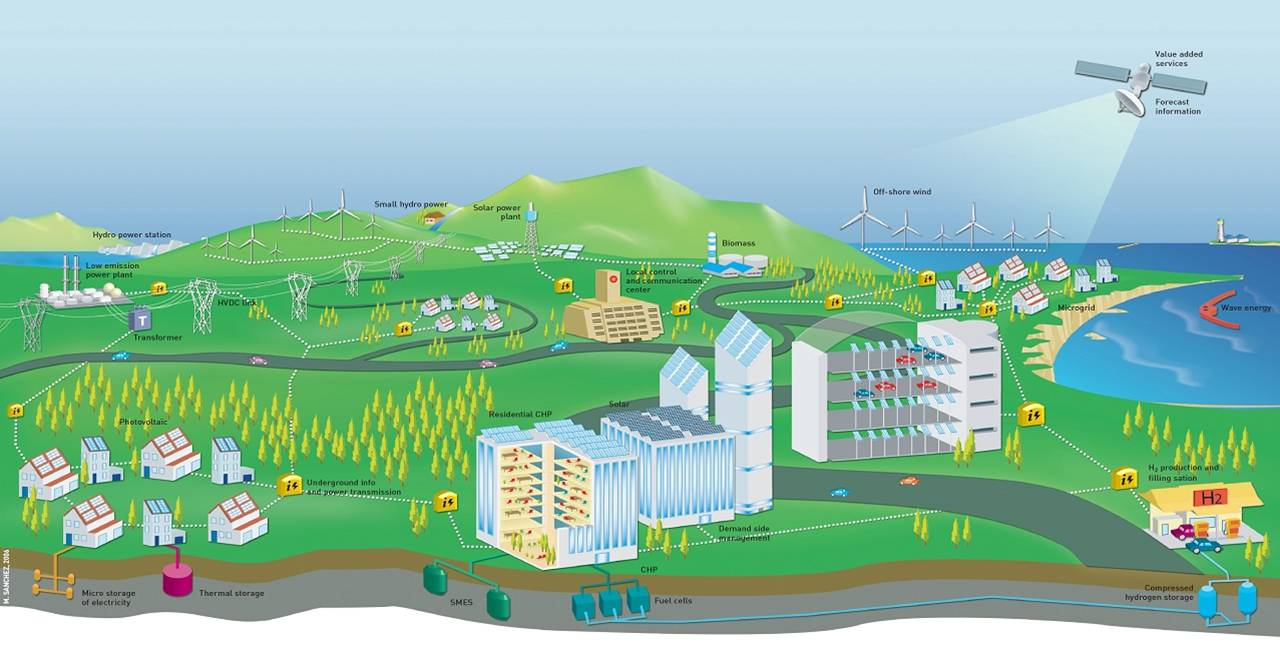
\includegraphics[scale=0.5]{figures/smart_grid_vision}
	\caption{Future network vision of the smart grids. Source: European Technology Platform for the Electricity Networks of the Future \cite{ETP_SG2006}}
	\label{fig:smart_grid_view}
\end{figure}


\section{Distributed energy resources}
\label{sec:DER}
This section explains the main characteristics of the current distributed energy resources (DER) and their benefits in the smart grids.
There are four kind of DER: distributed generation, storage units, demand side management and electric vehicles. Their common characteristic is that they are connected to the distribution grid: medium and low voltage networks.
Moreover, the recently growing of power converters has permitted to connect DC systems as batteries and DC generators to the AC grid. Besides, power converters can include control functions to optimize the operation of these resources in terms of active and reactive power, voltage, and frequency.

\subsection{Distributed generation}

Distributed generation (DG) is based on small but many generators dispersed in the territory. DG moves the consumption closer to production reducing the losses in the grid. 
There are two types of DG: dispatchable and non-dispatchable generators in function of their resource.

The most popular DG technology is the photovoltaic (PV) and this is non-dispatchable because it depends on the solar radiation. One of the key factors of its recent growth is that its efficiency is not very dependent on the scale of the system. Because of this, it can be installed in rooftops in households at a comparable costs of big PV power plants.

Micro-wind turbines are also a type of non-dispatchable DG but this technology is less mature and nowadays it is cost cannot compete with PV panels. Biomass gasifiers are an alternative to the PV systems and their advantage is that they are dispatchable renewable generators. Gasification is a thermochemical process that converts the biomass to a synthetic gas based on carbon-monoxide and hydrogen and syngas can be used in combustion engines or micro-gas turbines.

The economic feasibility of an energy generation project can be evaluated using various metrics but the levelized cost of energy (LCOE) is the most often used. LCOE permits to compare technologies considering all costs of these during their lifespan. The equation \ref{eq:LCOE} is the definition of LCOE and Lazard \cite{Lazard2014} presented this study to compare the costs of them in 2014.

\begin{equation}
LCOE = \frac{\sum_{t=0}^{T} \frac{I_t+O_t+M_t+F_t}{(1+r)^t}}{\sum_{t=0}^{T} \frac{E_t}{(1+r)^t}}
\label{eq:LCOE}
\end{equation}

\begin{itemize}
	\item $T$: life of the project [years]
	\item $t$: Year
	\item $E_t$: Energy produced for t [$\$$]
	\item $I_t$: Initial investment/cost of the system including construction, installation, etc. [\textdollar]
	\item $O_t$: Operation costs for t [\textdollar]
	\item $M_t$: Maintenance costs for t [\textdollar]
	\item $F_t$: Interest expenditures for t [\textdollar]
	\item $r$: Discount rate for t [$\%$]
\end{itemize}

\begin{figure}[h!]
	\centering
	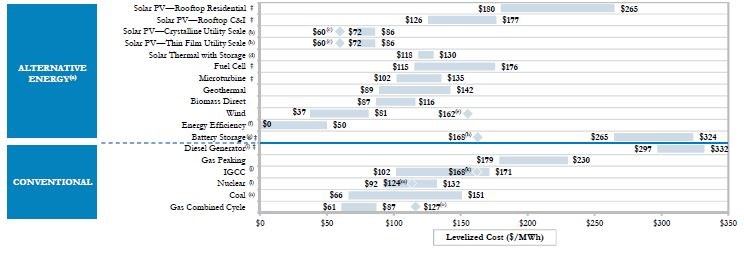
\includegraphics[scale=0.7]{figures/Captura_LCOE2}
	\caption{Unsubsidized levelized cost of energy comparison. Source: \cite{Lazard2014}}
\end{figure}

\subsection{Distributed energy storage}

Due to the growth of DG, the operation of distribution grids has become more complicated. One of the problems caused by DG is the frequency variations from non-dispatchable DG production fluctuations like PV reduction when clouds cover the panels. Nowadays this is a problem in some regions in the south of Germany with a high amount of PV generators.
One of the possible alternatives to solve the operation problems are the distributed energy storage units like electrochemical batteries, flywheels and ultracaps.

The benefits from storage are the increase of transport and distribution capacity, higher reliability, and peak demand reduction. Furthermore, the combination of storage units with DG could increase the capacity of the system to integrate more DG units in the distribution grids.

Nowadays there are different types of secondary batteries with different materials and advantages \cite{JoanMarc}:
\begin{itemize}
	\item \textbf{Lead acid} batteries are the most used technology; they are cheap and easy to recyclable. Their cathode is lead oxide, the anode is lead and electrolyte is aqueous sulfuric acid. Their drawbacks are the low energy density in terms of volume 25-50 Wh/kg and weight 50-90 Wh/l. Moreover, their lifespan is reduced due to the negative effects of deep discharges and it is arround 200-300 cycles in total life on average.
	\item \textbf{Nickel-metal hydride (Ni-MH)} batteries are based on nickel cadmium (Ni-Cd) ones but Ni-MH batteries use a hydrogen-absorbing alloy in the anode. This type of batteries offers higher energy densities of weight 70-100 Wh/kg instead of 40-60 Wh/kg of Ni-Cd, and also in terms of volume with 170-420 Wh/l instead of 50-150 Wh/l of Ni-Cd. The drawback of this technology is the self-discharging rate which is around 20$\%$ after 24 hours of a full charge and since then is 10$\%$ per month.
	\item \textbf{Lithium-ion (Li-ion)} batteries have not memory effect, their maintenance is low and their self-discharging rate is around 5$\%$ per month. The majority of these batteries the cathode is based on metal-oxide and their anode is mainly graphite. Their energy density is 75-200 Wh/kg and 250-620 Wh/l.
\end{itemize}

It seems clear that the lithium-ion batteries have better properties instead of lead acid and Ni-MH but their costs are still expensive. Moreover, their use in mobile applications such as electric vehicles can produce a second-life battery market. The usage of batteries reduces their capacity and it means that the EV owners could prefer to change the battery to avoid autonomy reduction. The batteries replaced from EV could have a second-life in stationary applications such as storage connected to the grid.

There are other storage technologies like flywheels, compressed air, pumped-storage, supercapacitors and hydrogen. But their usage in local electricity micro-markets is less useful. 
Technologies as flywheels and supercapacitors are more useful for technical services such as frequency grid support. 
Compressed air and pumped-storage are big infrastructures and the amount of energy that they manage is more than a neighbourhood could need. 
Finally hydrogen technologies are experimental and they are not ready for the market. For these reasons, the scope of this thesis is focused on electrochemical secondary Li-ion batteries.

\subsection{Demand side management}
The European Technology Platform defined the objective of DSM as: "Enable consumers' participation in the electricity market: Demand flexibility must be exploited to offer services to the different market participants enhancing consumer flexibility and adaptability, thus providing real-time optimisation of energy flows at local and global level. To this purpose, real-time metering data have the potential to facilitate active demand services." \cite{ETP_SG}

Smart grid technologies and demand side management (DSM), also known as demand response (DR), have been proposed as a technical solution to make demand more flexible and able to adapt to power generation and increase system efficiency, stability and reliability. DSM has been regarded as one of the most effective and efficient ways to solve problems associated with renewable energy integration into power system \cite{Sikai2009}. Shifting of load in certain optimal ways can contribute to various goals such as peak shaving and valley filling \cite{Kempton2005}. Responsive loads are one part of a DSM approach, which can offer different incentives and benefits to consumers in response to their flexibility, i.e. demand response (DR) \cite{Muratori}. DR is a cost effective technique and can be achieved by either price based or incentive based programs \cite{Wu}. The power grid has limited storage capabilities, so electricity generation and transmission must be continuously managed to match fluctuating demand \cite{Albadi}. Conventionally, this balance is maintained by power plants that remain on stand-by, ready to respond at desirable moment. DR programs can change consumption behavior by shifting loads to off-peak periods and participate in balancing of demand and supply \cite{Gottwalt}. Albadi and El-Saadany presented an overview of new flexible resources and defined DR programs and how electricity consumers can participate in those programs \cite{Albadi}. Others provided an overview of the evolution of the DR program and analysis of current opportunities \cite{Walawalkar}. Cappers et al. summarized the contribution of DR resources in the U.S., with the focus on performance of incentive-based DR programs in organized markets \cite{Cappers}. Kim and Shcherbakova examined central structural and behavioral obstacles to success of DR programs and defined some potential solutions which could greatly improve the functionality and success in the future \cite{Kim}. Ma and Alcadi assessed the realizable potential of DR for ancillary services (AS) in terms of economic value and implementation \cite{Ma}. Some authors proposed and explored a distributed direct load control approach for the large-scale residential DR \cite{Chen} and others investigated DR programs for residential appliances \cite{Vivekananthan} and \cite{Hamidi}, or electric heaters \cite{Ericson} and \cite{Saele}. Venkatesan et al. developed a model for DR to calculate the effect on the voltage profiles \cite{Venkatesan2011}, and others developed a model to assess the impact on both voltage profiles and grid losses of an electric distribution network \cite{Venkatesan2012} and \cite{Sundstrom}. 

The most costly part of the electricity demand is the one that occurs during the peak periods. Ultimate objective of DR programs is to reduce peak demand and programs are implemented so consumers can make decisions based on the information of price from the market. High price periods creates the opportunity for using electric vehicles with the vehicle-to-grid (V2G) services to provide required flexibility to the power system. V2G is the concept under which the power system can receive power from parked EVs. V2G services could be sold in an organized market as AS (regulation or spinning reserve), or as energy sales to the grid (peak power). The Federal Energy Regulatory Commission (FERC) reported a total potential DR contribution of about 37,500 MW in 2012 in the US \cite{Martini}. A total of 66 GW were under some form of control, making up 9$\%$ of total US national capacity in 2012. Response and the average estimated peak clipping was 8-11$\%$ while average estimated peak clipping in Europe in the same time was 6-13$\%$ \cite{Stromback}. 

Because of the plans of implementing smart grid technologies, some policy makers are anticipating that DR will be able to play a much bigger role in electricity markets in the near future \cite{Walawalkar}. Increased availability of DSM over the next 10 years will reduce peak demands, contribute to the deferral of new generating capacity, or improve operator flexibility in day-ahead or real-time time operations \cite{Stromback}. Ma, Callaway and Hiskens concluded that if 30$\%$ of conventional vehicles in the US were replaced by PHEVs, the total charging load would be around 140 GW, which accounts for 18$\%$ of the US summer peak load of 780 GW \cite{Ma2010}.

One of the most important challenges in the smart grid context is the employment of the necessary ICT infrastructure \cite{Vrba}. Authors proposed multi-agent system for various implementation, from calculating best solution for DSM program of PHEVs \cite{Vandael} to managing a power distribution system with PHEVs in smart grids \cite{Logenthiran}. Smart grid technology also enables bidirectional communication between the power system and the power consumer (EV owner or EV aggregator), so consumers can make decisions based on the information delivered to them. This communication infrastructure and protocols will greatly enhance DR capabilities of the whole system \cite{Fan}.

\subsection{Electric vehicles and grid integration}
The Electric Vehicles (EVs) are a distributed energy resource capable to control their consumption to charge batteries, to change their location and to discharge the battery if the system pays for this service. Before the expansion of EV the engineering has developed many models trying to create more or less realistic scenarios with EVs and they have been used to analyse their grid integration. This section exposes the variables implemented in the models to obtain the EV charging demand. These variables are: EV type, battery charging process, charging infrastructure, mobility and social variables, simulation techniques and the possible effects on power systems. 

\paragraph{EV type.}

From the point of view of EV charging demand, EVs main characteristics are the vehicle type: Plug-in Hybrid Electric Vehicle (PHEV) or Battery Electric Vehicle (BEV), battery capacity, battery technology, EV range and energy consumption. Amjad et al. \cite{Amjad2010} expose an  analysis about EV design considerations. Different authors only consider PHEV \cite{Watts-Transp,Clement2010,Peng2012,Chan2011,Sikai2010,Sortomme2011,Wang2011,Waraich2013}. Others only BEV \cite{Rahman1993,Valsera2011,Icai2010,Druitt2012,Loisel2014} or a combination of both \cite{Lyon2012,MaitraCIRED2009,Lopes2009Management,Soares2011}. Another option is to suppose average EV models, BEV and PHEV, with average characteristics like different authors do \cite{Watts-Transp,Icai2010,Soares2012}. Pang et al. \cite{Pang2012} simulate only two representative EV models: Chevy Volt (PHEV) and Nissan Leaf (BEV) and Valsera et al. \cite{Valsera2011} simulate Mitsubishi i-MiEV (BEV) only.

Soares et al. \cite{Soares2011} proposed a stochastic model with mobility variables, but the vehicle characteristics are determined by a Gaussian distribution with standard values for the capacity, energy consumption and charging power of EVs. 

The majority of papers simplify the EV model selection, but the capacity and the energy consumption are significant variables to be considered. The model presented proposes using real EV models and their technical data to define the battery capacity and energy consumption of each EV model. Moreover, the probability of each EV model is based on sales forecasting  \cite{EV_Forecast_FandS} to decide which EV model is more probable.

\paragraph{Battery and charging process.}

Regarding EV batteries, there are three variables linked: capacity (kWh), range (km) and energy consumption (kWh/km). \cite{Druitt2012,Tomic2007} consider the battery characteristics of real models and \cite{Loisel2014,Waraich2013,Metz2012,Lopez2013} consider average battery characteristics. Moreover, it is important to take into account the relation between the power consumed and the State-of-Charge (SoC). Valsera et al. \cite{Valsera2011} determine a relation between EV model, battery characteristics (Li-ion, 50 Ah, 16 kWh and 330 V) and its charging process. 

The charging process standards of IEC 61851 \cite{IEC61851-1} from Europe and SAE J1772 \cite{SAEJ1772} from the USA could also change the impact in the power system. Maitra et al. \cite{MaitraCIRED2009} compare the impact of each SAE standard. The voltage level in Europe for slow charges is 230 V and a maximum current of 16 or 20 A. In Belgium, houses have a protection up to 20 A \cite{Geth} and in Spain, the common protection is up to 16 A \cite{Valsera2011}. Valsera et al. use the power ratio of Mitsubishi i-MiEV when the initial SoC is 20$\%$ and the EV needs 4 hours to reach 100$\%$. Zhang et al. \cite{Zhang2011} use level 1 (120 V - 15 or 20 A) in the studio located in the United States. To compare, Grenier et al. \cite{GrenierNewZeland} use 230 V and 15 A and the study is located in New Zealand. The efficiency used in the studies is around 90$\%$, as Collins et al. proposed \cite{Collins1983} in 1983 and this assumption was recently confirmed by Shuang et al. \cite{Chan2011} and Clement et al. \cite{Clement2010,Clement2011}.

Different authors, such as Clement et al. \cite{Clement2010} and Guo et al. \cite{FactorAnalysisQinglai}, use constant power profiles. On the other hand, Maitra et al. \cite{MaitraCIRED2009} consider variable power during the charging profiles. Qian et al. \cite{Qian2011Modeling} propose a charging process model which links the power of the charger and SoC.  Gao et al. \cite{Chan2011_2} link the SoC and the charging time. Different authors use the specific EV charging profile of a real EV. For example, Qian et al. \cite{Qian2011Modeling} and Lojowska et al. \cite{Lojowska2011} use the charging profile of the Nissan Altra EV with a battery of 29 kWh, while Multin et al. \cite{Multin2012} use a three-phase charging profile of Opel Meriva, which has a battery of 16 kWh.

\paragraph{Charging infrastructure.}

Charging infrastructure parameters include the EV charging point's socket and availability to charge. The majority of works do not consider the EV infrastructure when calculating the EV charging demand. Inherent to this hypothesis is to neglect the effect of the queues at charging points by supposing there are enough charging stations, and the assumption of full compatibility between charging stations and EV connectors. Both could be reasonable in future scenarios with massive presence of EV, but could be a problem for fast chargers. Garc\'{\i}a-Valle et al. \cite{Garcia2009} introduce the queue theory with exponential distribution function to simulate EV charging time and relate it to the maximum charging power of the EV.

\paragraph{Mobility.}
Mobility is the third key point of EV charging demand. There is a strong link between energy consumption of EV and urban mobility. For example, Keirstead et al. \cite{Keirstead2012} reviewed the energy consumption in urban areas, including electric mobility.

Some authors employ the NHTS (National Household Travel Survey) to analyse the United States, such as \cite{Lyon2012,Zhang2011,FactorAnalysisQinglai,Kelly2012,Stephens_Michigan_2010,Weiller2011}. In the United Kingdom, studies use NTS (National Travel Survey) and UKTUS (United Kingdom Time Use Survey), for instance \cite{Sikai2010,Sikai2009,Sikai2011}. In Germany, there is the MID (\textit{Mobilit\"{a}t in Deutschland}) which Schroeder et al. \cite{Schroeder2012} and Loise \cite{Loisel2014} apply. The MON (\textit{Mobiliteitsonderzoek Nederland}) is utilised by Dutch studies, as Lojowska et al. cite \cite{Lojowska2011}. The DTU \textit{Transport, DTU. Transportvaneunders\o{}gelsen} is used by Jull et al. \cite{Juul2012} for a case study of Denmark. In the case of Spain, there are different databases, for example \textit{MOVILIA} for all of Spain such as Cruz et al. \cite{MiguelCruz2012} use and \textit{Dades B\`{a}siques de Mobilitat 2008} for Barcelona, like Valsera et al. use \cite{Valsera2011}

Metz \cite{Metz2012} makes use of the Deutsches Mobilit\"{a}tspanel to simulate 1000 mobility of household profiles and this includes day and time of departure and arrival, travel distance, vehicle used, and destination. Loise \cite{Loisel2014} makes projections of EV hourly charging profiles based on MID 2008.

The present work proposes that the reason of displacement be included to determine the destination and the instant of the day to displace. Due to that, it is possible to distinguish between professional and personal mobility.

\paragraph{Social.}
There are social variables related to the EV driver profile that could influence EV charging demand as GDP. Kelly et al. \cite{Kelly2012} analyse the EV charging demand considering the income, age and gender of drivers as well as the location (urban or rural). Sikai et al. \cite{Sikai2009} use the number of members of each household and the corresponding number of vehicles based on the UKTUS database. Valsera et al. \cite{Valsera2012} define the number of displacements, the number of houses, and the number of vehicles per house. The proposal of the present work is to combine these three approaches of the previous work to consider social aspects to calculate the EV charging demand.

\paragraph{Simulation techniques.}
To define the characteristics of simulations, there are different details set out by each author. The first one is the data processing, after that the emulation of parameters and lastly, the driver behaviour emulation.

Considering data processing, there are different types of simulation models to emulate the EV charging demand and the most used is agent-based. This type of model considers each EV driver autonomously defining the internal (e.g. energy consumption) and external (e.g. power demand to supply EV battery) variables. The bottom-up approach simulates the system coupling all the agents of the system. Different examples of agent-based and bottom-up approach studies are \cite{Stephens_Michigan_2010,Waraich_ETH,Galus2008}. On the other hand, the bottom-down approach simulates the EV driver behaviour with the average parameters \cite{Valsera2011,MaitraCIRED2009}.

Concerning the emulation of parameters, some models use deterministic variables and others stochastic ones. The deterministic approach considers just average values of parameters and stochastic models use probability distribution functions. The Monte Carlo technique is used to simulate stochastic variables in many applications and it is also used in modelling load, EV charging demand and distributed generation to determine their variability. The majority of studies set out a deterministic approach, but some of them include stochastic variables such as \cite{Sikai2010,Valsera2011,FactorAnalysisQinglai,Lojowska2011,Sikai2009,Sikai2011,Loisel2014}. Some of them use Monte Carlo techniques to simulate the total demand.

EV driver behaviour also influences the EV charging demand. This parameter is linked to time of day and location for EV charging, such as public stations between trips, at charging points at work or just home charging.

Venkatesan et al. \cite{Venkatesan2012} define user profiles related to estimated behaviour in the function of mobility, current electricity price and price forecasting. Waraich et al. \cite{Waraich_ETH} use microsimulation techniques to emulate the driver behaviour. Galus and Waraich \cite{Waraich_v2,Galus2009} use MATSim (Multi-Agent Transport Simulation) and this tool allows the creation of more than a million connections between agents in transport issues. Balmer \cite{BalmerMATSim} uses evolutionary algorithms; Hedegaard et al. \cite{Hedegaard66} propose using the Balmorel program to include distribution network, district heating, optimisation, taxes and geographical data.

\cite{Mohsenian2010} proposes including the game theory to simulate the interaction between agents and including sale of electricity with V2G service. Smith et al. \cite{Smith2011} use GPS data and EV metering to calculate the energy consumption and later to optimise the battery sizing of future PHEV.

The present work proposes combining some characteristics presented in literature. The methodology presented is a bottom-up approach to process the data with stochastic variables following the Monte Carlo formulation to emulate the parameters. And the driver behaviour is defined in function of the range anxiety, the mobility needs and the energy price.

\paragraph{Power system impact.}
Possible effects on power networks caused by EVs are related to power quality or grid saturation. The majority of studies analyse the voltage drop or transformer load, like Valsera et al. \cite{Valsera2011,Valsera2012}. Clement et al. \cite{Clement2010} include Joule losses and Maitra et al. \cite{MaitraCIRED2009} include overloading and unbalances. Kleiwegt et al. \cite{Kleiwegt2012} propose a methodology to detect overloads in the course of a year. Moreover, vehicle-to-grid possibility is analysed in many studies such as \cite{Kempton2005, Tomic2007, Zakariazadeh2014}. Another possible impact on the power system is economic and this is reviewed by Dallinger et al. \cite{Dallinger2012}. The present work analyses the distribution network in terms of the HV/MV and MV/LV transformer capacities and the voltage of each node.

\section{Electricity markets}
\label{sec:markets}
%De-regulation
Electricity markets are described as a very important zone in the smart grid plane. Markets are a way to organize the distribution of commodities in an efficient way when conditions enhance perfect competition between the actors. However, electricity is not a simple commodity. In order to ensure  reliable and continuous delivery of significant amounts of electricity, the system needs bulk generation plants, transmission and distribution grids and different control and monitoring functions to keep the system technically feasible. The simple fact that there is a limited amount of storage capability (due to technical and economic reasons) in the grids, makes the electricity market unique. The technical differences of the commodity "electricity" have a profound effect on the organization and the rules of electricity markets.

The main objective of electricity markets is to introduce competition between agents like generators and retailers and then to ensure the minimum electricity price for customers. Four models of competition has been discussed \cite{Economics_Kirschen} and listed below:

\begin{enumerate}
	\item Monopoly
	\item Purchasing agency
	\item Wholesale competition
	\item Retail competition
\end{enumerate}

\textbf{Monopoly} is the most regulated model and it has not competition. The rest of the markets are known as de-regulated but none of them are purely de-regulated. 

In a monopoly the traditional monopolistic utilities; state vertically integrated companies, have the control on generation, transmission, and distribution of electricity, as is shown in Figure \ref{fig:monopoly}. The electricity price of consumers is regulated by a governmental agency or a ministry, and the remuneration for those utilities was supervised by the state. This model was the unique proposal until 80's decade when the Chicago Boys, a Chilean economist group from the Department of Economics of the University of Chicago, applied their theories of privatization and de-regulation in the electric power system of Chile. The World Bank introduced hybrid models in many countries of Latin America with limited success. In 90's, the UK privatised the power system in UK and in the Commonwealth countries. In 1997, Rodrigo Rato, as Minister of economy and finances with Jose Maria Aznar as prime minister, privatised the power industry in Spain and created the Spanish electricity market.

\begin{figure}[h!]
	\centering
	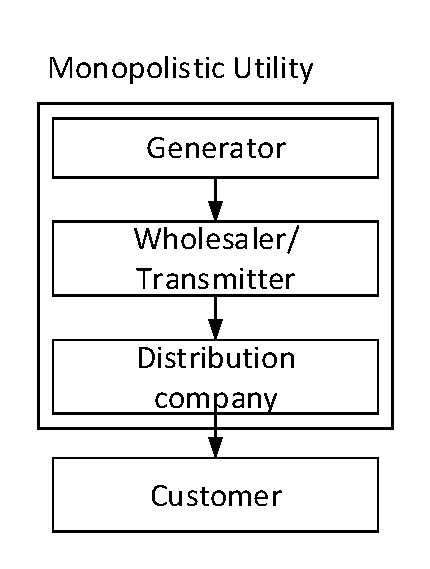
\includegraphics[scale=0.7]{Visios/Market_competition_Monopoly}
	\caption{Monopoly  model. Source: \cite{Economics_Kirschen}}
	\label{fig:monopoly}
\end{figure}

\textbf{Purchasing agency} model is the first de-regulated model which has a purchasing agency. In this model, independent power producers (IPP) are integrated in the system, competing between each other. The utility acts as a wholesale purchasing agent buying the energy from the best generator offers and it sells the electricity in a monopoly transmission and distribution system to the consumers. The electricity prices are regulated because the distribution companies have the monopoly. The figure \ref{fig:purchasing} shows the purchasing agency model where the IPPs compete to sell the energy to the Discos through the wholesale purchasing agency.

\begin{figure}[h!]
	\centering
	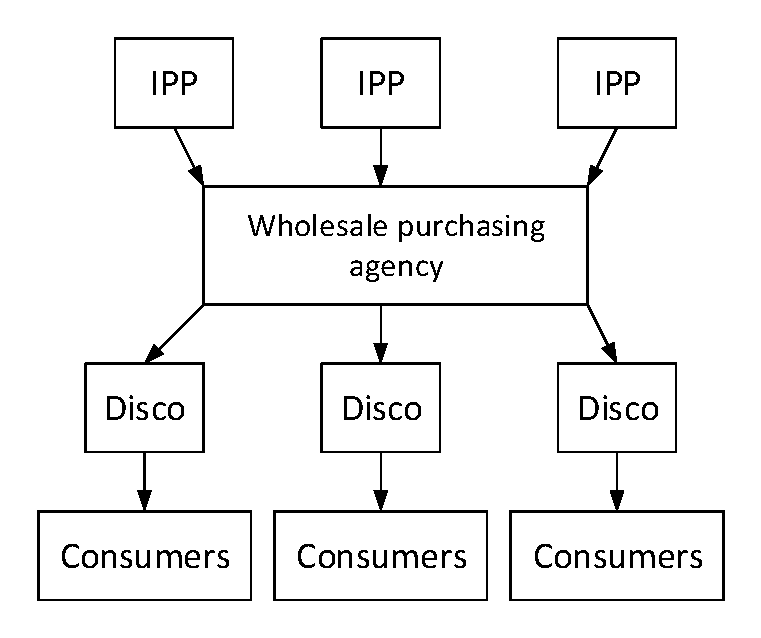
\includegraphics[scale=0.7]{Visios/Market_competition_Purchasing_agency}
	\caption{Purchasing agency  model. Source: \cite{Economics_Kirschen}}
	\label{fig:purchasing}
\end{figure}

\textbf{Wholesale competition model} is hybrid because there is competition in the generation level but not in the retail level. In this model distribution companies purchase the electricity directly from generating companies in a wholesale electricity market that is mainly taking place on the transmission level. Whereas distribution companies remains in a monopoly in the retail level because they purchase the energy to sell them to consumers, as is shown in Figure \ref{fig:wholesale}. Large consumers are the exception of this system because they can purchase electricity directly in the market.

\begin{figure}[h!]
	\centering
	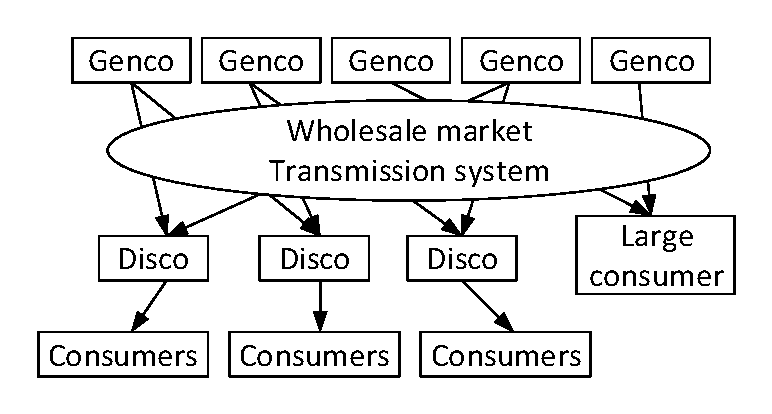
\includegraphics[scale=0.7]{Visios/Market_competition_Wholesale_competition}
	\caption{Wholesale competition model. Source: \cite{Economics_Kirschen}}
	\label{fig:wholesale}
\end{figure}

\textbf{Retail competition} model allows all consumers to choose their supplier freely. In practice, only large consumers will participate in the wholesale market directly. To enhance the complex participation on the electricity market of small and medium consumers, those consumers are purchasing it's electricity via retailers that are operating on the wholesale market, as is shown in Figure \ref{fig:retail}. In this model the distribution activity is separated to the energy sales to create competition in the retail side with the objective to reduce the electricity price of consumers. For physical reasons the transmission and distribution remains as monopolies regulated by the governmental agencies and their costs are charged to the consumers.

\begin{figure}[h!]
	\centering
	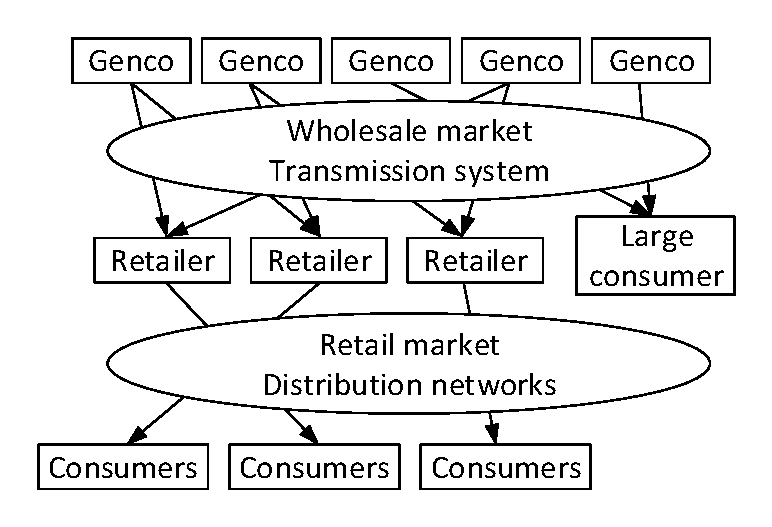
\includegraphics[scale=0.7]{Visios/Market_competition_Retail_competition}
	\caption{Retail competition  model. Source: \cite{Economics_Kirschen}}
	\label{fig:retail}
\end{figure}

%\subsection{De-regulated system}
The European Union obliged all EU members to de-regulate the market, to create a retail competition and to divide the vertical companies in each activity. Due to that, nowadays big energy companies are holdings of different companies such as generation company, distribution company and retail company. Transmission and distribution activities are regulated due to them are natural monopolies. 
Transmission companies are used to being unique for each country as REE in Spain or RTE in France, or divided in areas like Germany which has four transmission companies: Tennet, Amprion, EnBW and Elia. The association ENTSO-E aggregates all of European transmission companies. 
In contrast, distribution companies are more sub-divided by areas, they control the distribution networks including medium and low voltage grids. Moreover, there are much more distribution companies instead of transmission ones.

%Day-ahead & Europe
Nowadays, Electricity prices in Europe are set on a daily basis for twenty-four hours of the following day in what is called the Daily market or Day-ahead market. The power price is determined by the balance between supply and demand. Factors such as the weather or power plants not producing to their full capacity can impact power prices.
The figure \ref{fig:bids-offers} shows the demand and supply curves, and price and volume of energy are determined by the point at which the supply (yellow) and demand (blue) curves meet, known as marginal price. This is the basic concept of pool markets. 

Some day-ahead markets accept complex offers as in the Spanish one. In this type of markets generators can establish conditions to deliver the energy such as the minimum income for all day or the ramp-up/ramp-down limitations, both only for generators. 
Due to complex offers, the marginal price increases because some cheap generators are substituted for more expensive ones. The red curve shown in the figure \ref{fig:bids-offers} are the generators with no issues with the final matching point, hence the final price is higher. 

\begin{figure}[h!]
	\centering
	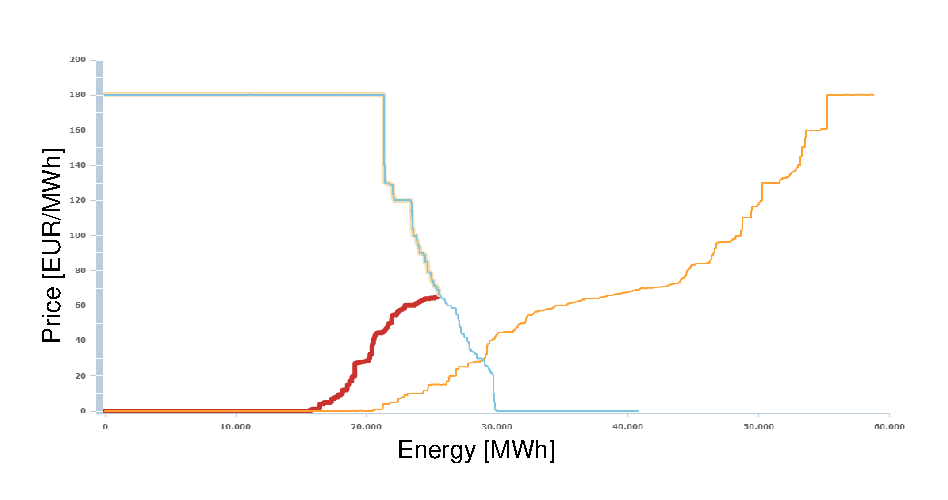
\includegraphics[scale=0.9]{Visios/Captura_mercado_diario}
	\caption{Curves of supply and demand on energy. 22nd of October of 2014, hour 20 in the OMIE day-ahead market. Source: \cite{OMIE_22102014}}
	\label{fig:bids-offers}
\end{figure}

\subsection{Spanish electricity market}
The Spanish electricity market is composed by two economic and six technical markets. Figure \ref{fig:Spain_structure} shows the responsible of each market; market or system operator, and the day when the market is closed; D-1 (a day before) and D (the day when the demand occurs). Portugal and Spain are in the same electricity market and the market operator is OMIE.

\begin{figure}[h!]
	\centering
	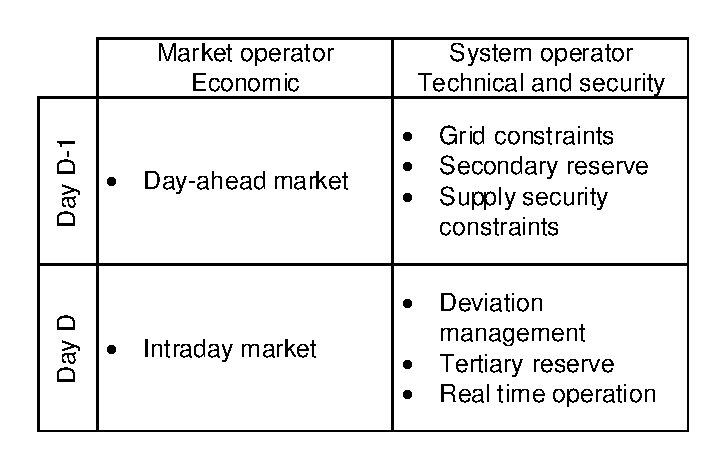
\includegraphics[scale=0.7]{Visios/Spanish_market_structure}
	\caption{Spanish market structure. Source: }
	\label{fig:Spain_structure}
\end{figure}

The most important electricity market is the day-ahead market due to the amount of energy negotiated. 
In 2013 the Spanish day-ahead market negotiated 185.1 TWh, the intra-day market managed 34.6 TWh and in all technical markets arranged 25.0 TWh for the Spanish side \cite{REE_2013}. 
Furthermore, the  Figure \ref{fig:price2013} shows the average electricity prices in 2013 per month and the corresponding market. 
Moreover, it shows that technical and capacity costs are quiet constant during the year. In contrast, the day-ahead and intra-day markets (blue bars) are the cause of the final price variations.

\begin{figure}[h!]
	\centering
	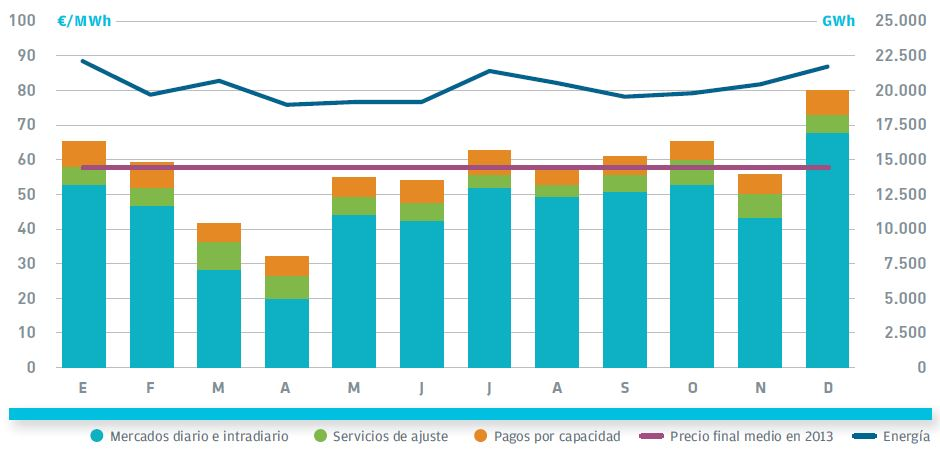
\includegraphics[scale=0.54]{figures/Captura_preu_final_REE_2013}
	\caption{Average final price and energy of Spanish side in 2013. Blue bars: day-ahead and intra-day, green bars: deviations adjustments, orange bars: capacity payments, purple line: average electricity price in 2013 and blue line: Energy. Source: \cite{REE_2013}}	
	\label{fig:price2013}
	
\end{figure}

\subsection{European market (EUPHEMIA)}
%Treball master Energy markets
The international exchanges between different power systems are a very important issue in their operation. International connections allow to make offers or bids between different systems and to increase the competition between agents increasing the number of generators and retailers. Furthermore, the connection between different systems permits to increase the renewable generators because the system can sell the surplus of energy to other markets.

The key question of international exchanges is how to increase the competition between generators in an easy way. Since the beginning of 2014, capacity allocation rules between Spain and France were very complicated. 

With the aim of increasing the competition in all the European energy markets, the project called Price Coupling of Regions (PCR) has analysed different alternatives and as a result, the project designed the algorithm to couple all European markets. It is called EUPHEMIA (acronym of Pan-European Hybrid Electricity Market Integration Algorithm) \cite{euphemia}.

The involved market operators are: 
\begin{itemize}
	\item EPEX Spot: France, Germany, Austria and Switzerland.
	\item APX: United Kingdom and Nederlands
	\item Belpex: Belgium 
	\item Nord Pool Spot: Norway, Sweden, Denmark, Finland, Estonia, Latvia and Lithuania 
	\item OMIE: Spain and Portugal 
	\item Mercatoelettrico (GME): Italy
	\item OTE: Czech Republic
	
\end{itemize}

Since February of 2014, the coupled markets are: APX, Belpex, EPEX SPOT and Nord Pool, which corresponds to North-Western Europe (NEW) day-ahead price coupling project. Later on, South-Western Europe (SWE) project: France, Spain and Portugal will be coupled. 

The Slovak, Hungarian and Romanian market operators / power exchanges together with the Czech market operator are currently implementing a coupling solution for their day-ahead electricity markets (4M MC project) relying on the Price Coupling of Regions (PCR) solution, which has been operating the NWE and SWE regions since 4 February 2014.

\subsection{Electricity micro-markets}
\label{sec:SoA_mm}
%Problem presentation
After the review of electricity markets is necessary to detect their problems. 
Nowadays, the main problem of current electricity markets based on the pool system is the participation of renewable generators without operation costs, like wind turbines and photovoltaic systems.
These generators offer energy at price zero expecting that the price matched will be higher than zero. When the amount of energy at price zero is not significant, the prices remain similar to those without renewable generators. But if the amount of energy offered by generators without operational costs is equal to or higher than the energy consumed, then the price matched is zero and the renewable generators cannot recover the initial investment. Figure \ref{fig:OMIE_02022013} shows the day-head market prices on 2nd of February of 2013 where the price in Spain was zero from hour 3 until hour 18.

\begin{figure}[h!]
	\centering
	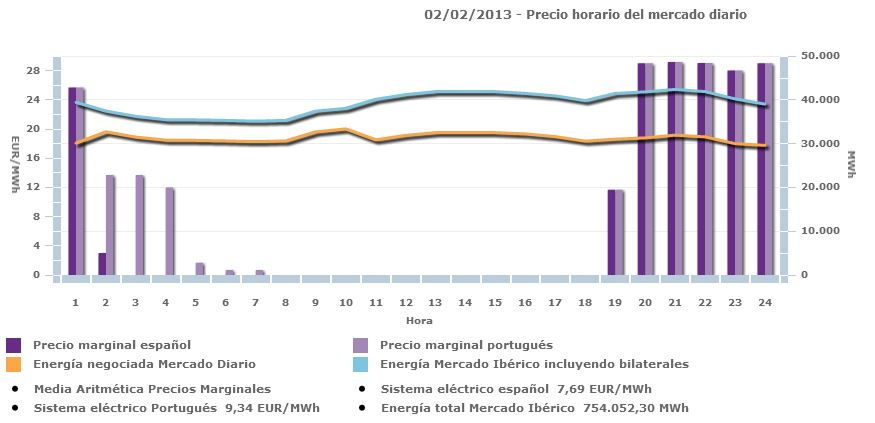
\includegraphics[scale=0.6]{Figures/Captura_mercat_diari_febrer2013}
	\caption{Day-ahead prices and energy purchased in 2nd of February of 2013. Source: \cite{OMIE_02022013}}
	\label{fig:OMIE_02022013}
\end{figure}

%The second problem-Network constraints
Moreover, the second problem in the day-ahead markets is that the network constraints provoke that some configurations established in the market are not technically feasible. Due to this situation final energy prices increase in technical markets. 

%Alternatives: grid expansion/micro-markets
There are different proposals to solve the problems of renewable generators integration in the market. The basic solution is to expand the grid to ensure the transmission of energy but this solution is expensive and complicated to implant due to the NIMBY (Not In My Back Yard) effect. The alternative is to create micro-markets which consider network constraints to avoid inefficiencies in the wholesale market. Because of the scale of the problem in a micro-market, the optimal power flow can be calculated.

%micromarket definition
A micro-market is the aggregation of local generators and demands from a neighbourhood
which permits solving the network constraints locally.
Furthermore, a micro-market could permit creating offers and bids to participate in the wholesale market considering the network constraints.

%clearing procedures
Clearing procedures could be cooperative based on costs or competitive based on offers and bids. The advantage of procedures based on costs is that the aggregator could determine the minimum operation configuration easily. 
But the drawback is that systems with multiple generator owners can be easily manipulated by some of them declaring different costs than the real ones. 
Whereas the advantage of competition systems is that it is not necessary to declare costs of each generator and then the operation point can be determined based on offers, bids and grid connection point, if network constraints are considered. 
While the drawback of competition systems is that systems with few participants could be controlled by generators with an elevated share in the market.
%final conclusion after the comparison
As a conclusion, cooperative systems seem to be more appropriate for single-owner systems and competition systems are more suitable for multiple-owner systems with enough participants to avoid manipulations \cite{Microgrids_Nikos}. 
%What they do in the micromarket proposed
In the micro-market proposed, the consumers or the market aggregator on behalf of them, and the generators have to send bids and offers respectively to the market aggregator. And then the market aggregator can determine the clearing point. 

%advantatges
The micro-market structure has the advantage against centralized control systems in that it permits integrating different owners with total privacy. Furthermore, the benefits of micro-markets in distribution systems are:

\begin{itemize}
	\item Optimal power flow can be implemented ensuring lower costs and losses.
	\item Storage units can be operated optimally considering economic and technical constraints.
	\item They have higher resilience and they can react easily under unexpected situations.
	\item Power quality can be increased with local controls.
\end{itemize}

The micro-markets characteristics are:
\begin{itemize}
	\item Micro-markets induce competition and they are non-discriminatory.
	\item The wholesale market can participate through the virtual market agent.
	\item The objectives of buyers and sellers are purely economics.
	\item The auction can include the grid constraints to ensure a feasible clearing point. 
	\item Demand response can be easily implemented in the micro-market and demand agents can send offers to the micro-market.
\end{itemize}

% MM_16 literal
The literature about micro-markets reviewed is very brief and this is a topic very novel because the technology that enables is very recent. Tables \ref{table:MM_ref1} and \ref{table:MM_ref2} summarise the most important contributions from the literature.

\begin{landscape}
\begin{table}[htbp]
	\centering
	\caption{References in micro-markets design - Part I}
	\label{table:MM_ref1}
	\begin{tabular}{lll}
		\cline{1-3}
		{\bf Reference} & {\bf Contributions}                                                                                                                                                                                                                                                                                                                                                                               & {\bf Year} \\ \cline{1-3}
		\cite{MM_01} & \begin{tabular}[c]{@{}l@{}}Decentralized EMS for DSM. \\ House Level.\\ No optimization.\\ Each device reduce the consumption in terms of \\ the cost of the general function.\\ The micro market controller gives the priority to the highest load.\end{tabular} & 2014 \\
		\cline{1-3}
		\cite{MM_03} & \begin{tabular}[c]{@{}l@{}}To include the participation of DER and end-consumers in system balancing. \\ Real-time prices.\\   Demand response. \\ Ecogrid Project. \end{tabular}                                                                                                                                                                                                                    & 2013 \\
		\cline{1-3}
		\cite{MM_05} & \begin{tabular}[c]{@{}l@{}} Demand response. \\ Real demonstration.\\ PowerMatching City project.\\ \end{tabular}                                                                                                                                                                                                                                                                                       & 2013  \\
		\cline{1-3}
		\cite{MM_12} & \begin{tabular}[c]{@{}l@{}}"Local energy markets allow an efficient allocation and \\ distribution of energy from local sources to nearby  households."\\ The influence of anonymization methods on local energy markets.\\ It includes a local market operator.\\  Discret time double-auction, where the market is cleared at fixed points in time.\\ Anonymous Auctions\end{tabular} & 2013 \\ \cline{1-3}
	\end{tabular}
\end{table}
\end{landscape}

\begin{landscape}
	\begin{table}[htbp]
		\centering
		\caption{References in micro-markets design - Part II}
		\label{table:MM_ref2}
		\begin{tabular}{lll}
			\cline{1-3}
			{\bf Reference}       & {\bf Contributions}                                                                                                                                                                                                                                                                                                                                                                                                                                                                                                                                                                                                                                                                                                                                    & {\bf Year}  \\
			\cline{1-3}
			\cite{MM_13}       & \begin{tabular}[c]{@{}l@{}}Each microgrid can trade with its neighborhoods \\ and thus achieve a welfare increase from making use of its.\\ Comparative advantage on power generation during a certain period of time\end{tabular}                                                                                                               & 2014    \\
			\cline{1-3}
			\cite{ampatzis2014} & \begin{tabular}[c]{@{}l@{}} A shorter trading horizon in the scale of minutes.\\ Continuous double-sided auction with private information.\\ Discriminatory pricing.\\ No big participants.\\ The market clears continuously until the end of the trading period so that\\ the participants have time to improve their bids if initially they are unmatched.\\ A fifteen minute trading horizon is proposed for a dispatch of five  minutes.\\ No OPF.\\ \end{tabular}                                                                                                                                                                                                                                                    & 2014  \\
			\cline{1-3}
			\cite{MM_20}       & \begin{tabular}[c]{@{}l@{}}Micromarket requirements:\\   market clearing, converging algorithms, non-repudiation and clear rules\\ Macromarkets recuces the risks.\\     Advantatges:\\ -It reduces consumer buy-in to and acceptance of smart energy.\\ -It slows the ability of the system to consume new technologies and new interactions \\   It reduces the willingness of new participants to enter the market.\\ Disadvantatges:\\     -Additional complexity\end{tabular} & 2011 \\
			\cline{1-3}
		\end{tabular}
	\end{table}
\end{landscape}

According to Ampatzis et al. \cite{ampatzis2014} micro-market depends on:
\begin{itemize}
	\item Configuration of the local power system
	\item Objective of the stakeholders involved
	\item Characteristics of market participants
\end{itemize}

And the factors that influence on the design of micro-markets are:
\begin{itemize}
	\item Degree of competition: a big player can control the energy price against the majority
	\item Trading horizon: the day-ahead market requires good precision in the forecasting. In contrast, real-time markets in the scale of minutes is a balancing mechanism.
	\item Dispatch intervals: Short dispatch intervals reduce the deviations from the forecasted energy.
	\item Cost structure for the participants
\end{itemize}

Generation and consumption coordination can be towards numerous directions according to \cite{ampatzis2014}, such as:
\begin{itemize}
	\item voltage support
	\item frequency control
	\item provision of active power reserves
	\item ancillary services
\end{itemize}

\section{New agents}
\label{sec:SoA3}
As it has been said previously, there are new agents in the grid like Microgrids and virtual power plant operators, and EV aggregators with new interests and capabilities. The creation of these agents is due to the expansion of ICT technologies and smart meters, and decrease of DER costs.

\paragraph{Microgrids and Virtual Power Plants}
The main objective of microgrids and virtual power plants (VPP) is to manage multi-generation systems concentrated or dispersed in the grid respectively.

Their origin is the DG cost reduction, hence electricity grid will have a lot of DG spread in the territory. To reduce DG operation costs they could decide to act together. In small-scale they will be known as microgrids and the large-scale of microgrids are virtual power plants (VPP).

Microgrids are small-scale low voltage networks designed to supply electrical and heat loads for a small community. Microgrids essentially conglomerates DG units and loads at distribution level \cite{Chowdhury}.

Braun \cite{braun2009provision} defined a VPP like an information and communication system that aggregates Controllable Distributed Energy (CDE) units or Active Customer Networks (ACN) by direct centralised control. CDE units can be DG, Energy Storage Systems, Controllable Loads or Electric Vehicles. ACN are defined like private networks with CDE units able to control active and reactive power at the connection point. The scale of VPP is bigger than microgrids and VPP are not necessary connected to a common LV grid. 

For both cases, it is necessary an agent who is the responsible of the operation. This agent have to send the messages with the other grid stakeholders as DSO or TSO, market operator and regulator.

\paragraph{EV aggregators for more EV integration}
In the same manner, EVs will need an agent which aggregates all of them to buy their energy in the wholesale market, to manage the charging stations and optimizing their charge to reduce the impact on power system as it is explained in chapter \ref{ch:EV}. Gomez et al. \cite{Gomez} exposed diverse regulations and business models around the EV and their charging infrastructure.

\begin{itemize}
	\item Electric vehicles (EVs) aggregators to control EVs in terms of charging/discharging and addition services as charging points management.
	\item Energy service providers 
\end{itemize} 

\section{Smart Grid Architecture Model}
\label{sec:SGAM}

The Smart Grid Architecture Model (SGAM) framework has been developed by the Joint Working Group on standards for Smart Grids from CEN/CENELEC/ETSI. Its methodology is intended to present the design of smart grid use cases by a holistic architecture definition of an overall Smart Grid infrastructure.

Apart of addressing the system architecture through reference architecture, it is also overarching standardisation process. The major elements of the described reference architecture are:
\begin{enumerate}
	\item A high-level framework model (European Conceptual Model) that is an adapted version of the US NIST (National Institute of Standards and Technology) model.
	\item SGAM Framework as a three dimensional model with interoperability layers and smart grid zones and domains, that is assisting the architecture design of smart grid use cases
	\item Representations of stakeholder views of smart grids.
\end{enumerate}

\paragraph{Domains.} The different domains are standing for the power system equipments and energy conversion divided in following subgroubs, enumerated from 1 to 5:

\begin{description}
	\item[1. Bulk Generation.] This domain is representing the bulk generation of electricity by power plants. It is representing the "classical" power system generation, such as by thermal, nuclear and hydro power plants as well as big sized renewable generation like off-shore wind farms and large scale photovoltaic (PV) power plants. They are typically connected to the transmission system.
	\item[2. Transmission.] This domain is representing the necessary infrastructure and organization for transmission of large powers over long distances.
	\item[3. Distribution.] This domain is representing infrastructure and organization for distribution of electricity to final customers. 
	\item[4. DER.] This domain represents the distributed energy resource generation, typically using small-scale generation technologies based on renewable energy resources. The range of such generators is typically from 3 kW up to  10 MW, they are connected directly to the distribution grid and can be controlled by the distribution system operator. 
	\item[5. Customer Premises.] This domain includes the industrial, commercial and home facilities where the electricity users interact with the distribution system. In the classical approach here are the consumers placed (households, industrial plants, shopping malls, etc.). In the prosumer approach, also small scale generation, electric vehicles, demand response, batteries etc. can be hosted.
\end{description}

\paragraph{Zones.} The Smart Grid Plane is also divided in different zones described below. The idea behind the introduction of zones in the plane is the fact that there are in modern power systems different viewpoints of the same basic processes. So, the the processes depend on the zone described differently without interfering the functionality of other zones. Apart of the process zone, all zones are representing information management. The zones are enumerated from a. to e. as follows:

\begin{description}
	\item[a. Process.] This zone includes both primary equipment of the power system like generators, transformers, substation equipment, transmission and distribution lines, loads. It represents basically the classical understanding of a power system. This includes also the equipment for the physical energy conversion between electricity, solar, heat, water, wind etc.
	\item[b. Station.] This zone represents the aggregation level for fields, for example for data concentration or substation automation.
	\item[c. Operation.] This zone in hosting the power system control and operation for the respective domains. For example, for the distribution domain the distribution management systems (DMS), for the generation and transmission domain the energy management systems (EMS), etc. 
	\item[d. Enterprise.] In this zone, the commercial and organizational processes of an enterprise, including services (staff training, customer relation management, billing and procurement, etc.) and asset management of the different actors. 
	\item[e. Market.] Finally, in this zone the possible market involvement of the different actors along the whole production chain is reflected. 
\end{description}

\paragraph{Interoperability dimension.} To complement the Smart Grid Plane, five abstract layers are added in order to represent the different viewpoints of the system. It will provide a clear presentation and simple handling of the presented architecture model, enabling the interoperability of this system. The different layers are specified as follows, enumerated from A to E: 

\begin{description}
	\item[A. Component.] In this layer, the physical distribution of all participating components in the smart grid are represented (sensors and actors): system actors, applications, power system equipment, protection and control devices, network infrastructure, etc. 
	\item[B. Communication.] This layer describes the communication protocols and mechanisms for exchange of information (connectivity). This layer is important to guarantee the interoperability. 
	\item[C. Information.] This layer is representing data that is used and exchanged between functions, services and components: power quality data, power flow, protection, data from DERs, customers and meter data, etc.
	\item[D. Function.] This layer contains the definition of the functions and services and their relationships from an architectural viewpoint.  It describes how the function or service are performed independently from actors and physical implementations, systems or components.
	\item[E. Business.] This layer is representing the business view of the smart grid. It can be used to represent the market, regulatory and economic structures as well as policies, business models, products and services of market participants. 
	
\end{description}

The SGAM is a very holistic view of the whole smart grid architecture, including widespread viewpoints on the power system. It is a fact that the classical approach for power engineering  (this are all the domains of the process zone of the component layer) is enriched by the information management zones and all the other layers. The complementing zones and layers are defined in order to have a clear description and to enable the interoperability. This does not mean that they did not exist before; they were integrated in the power system engineering approach. By separating them, clarity of the solution is enhanced.

\begin{figure}[h!]
	\centering
	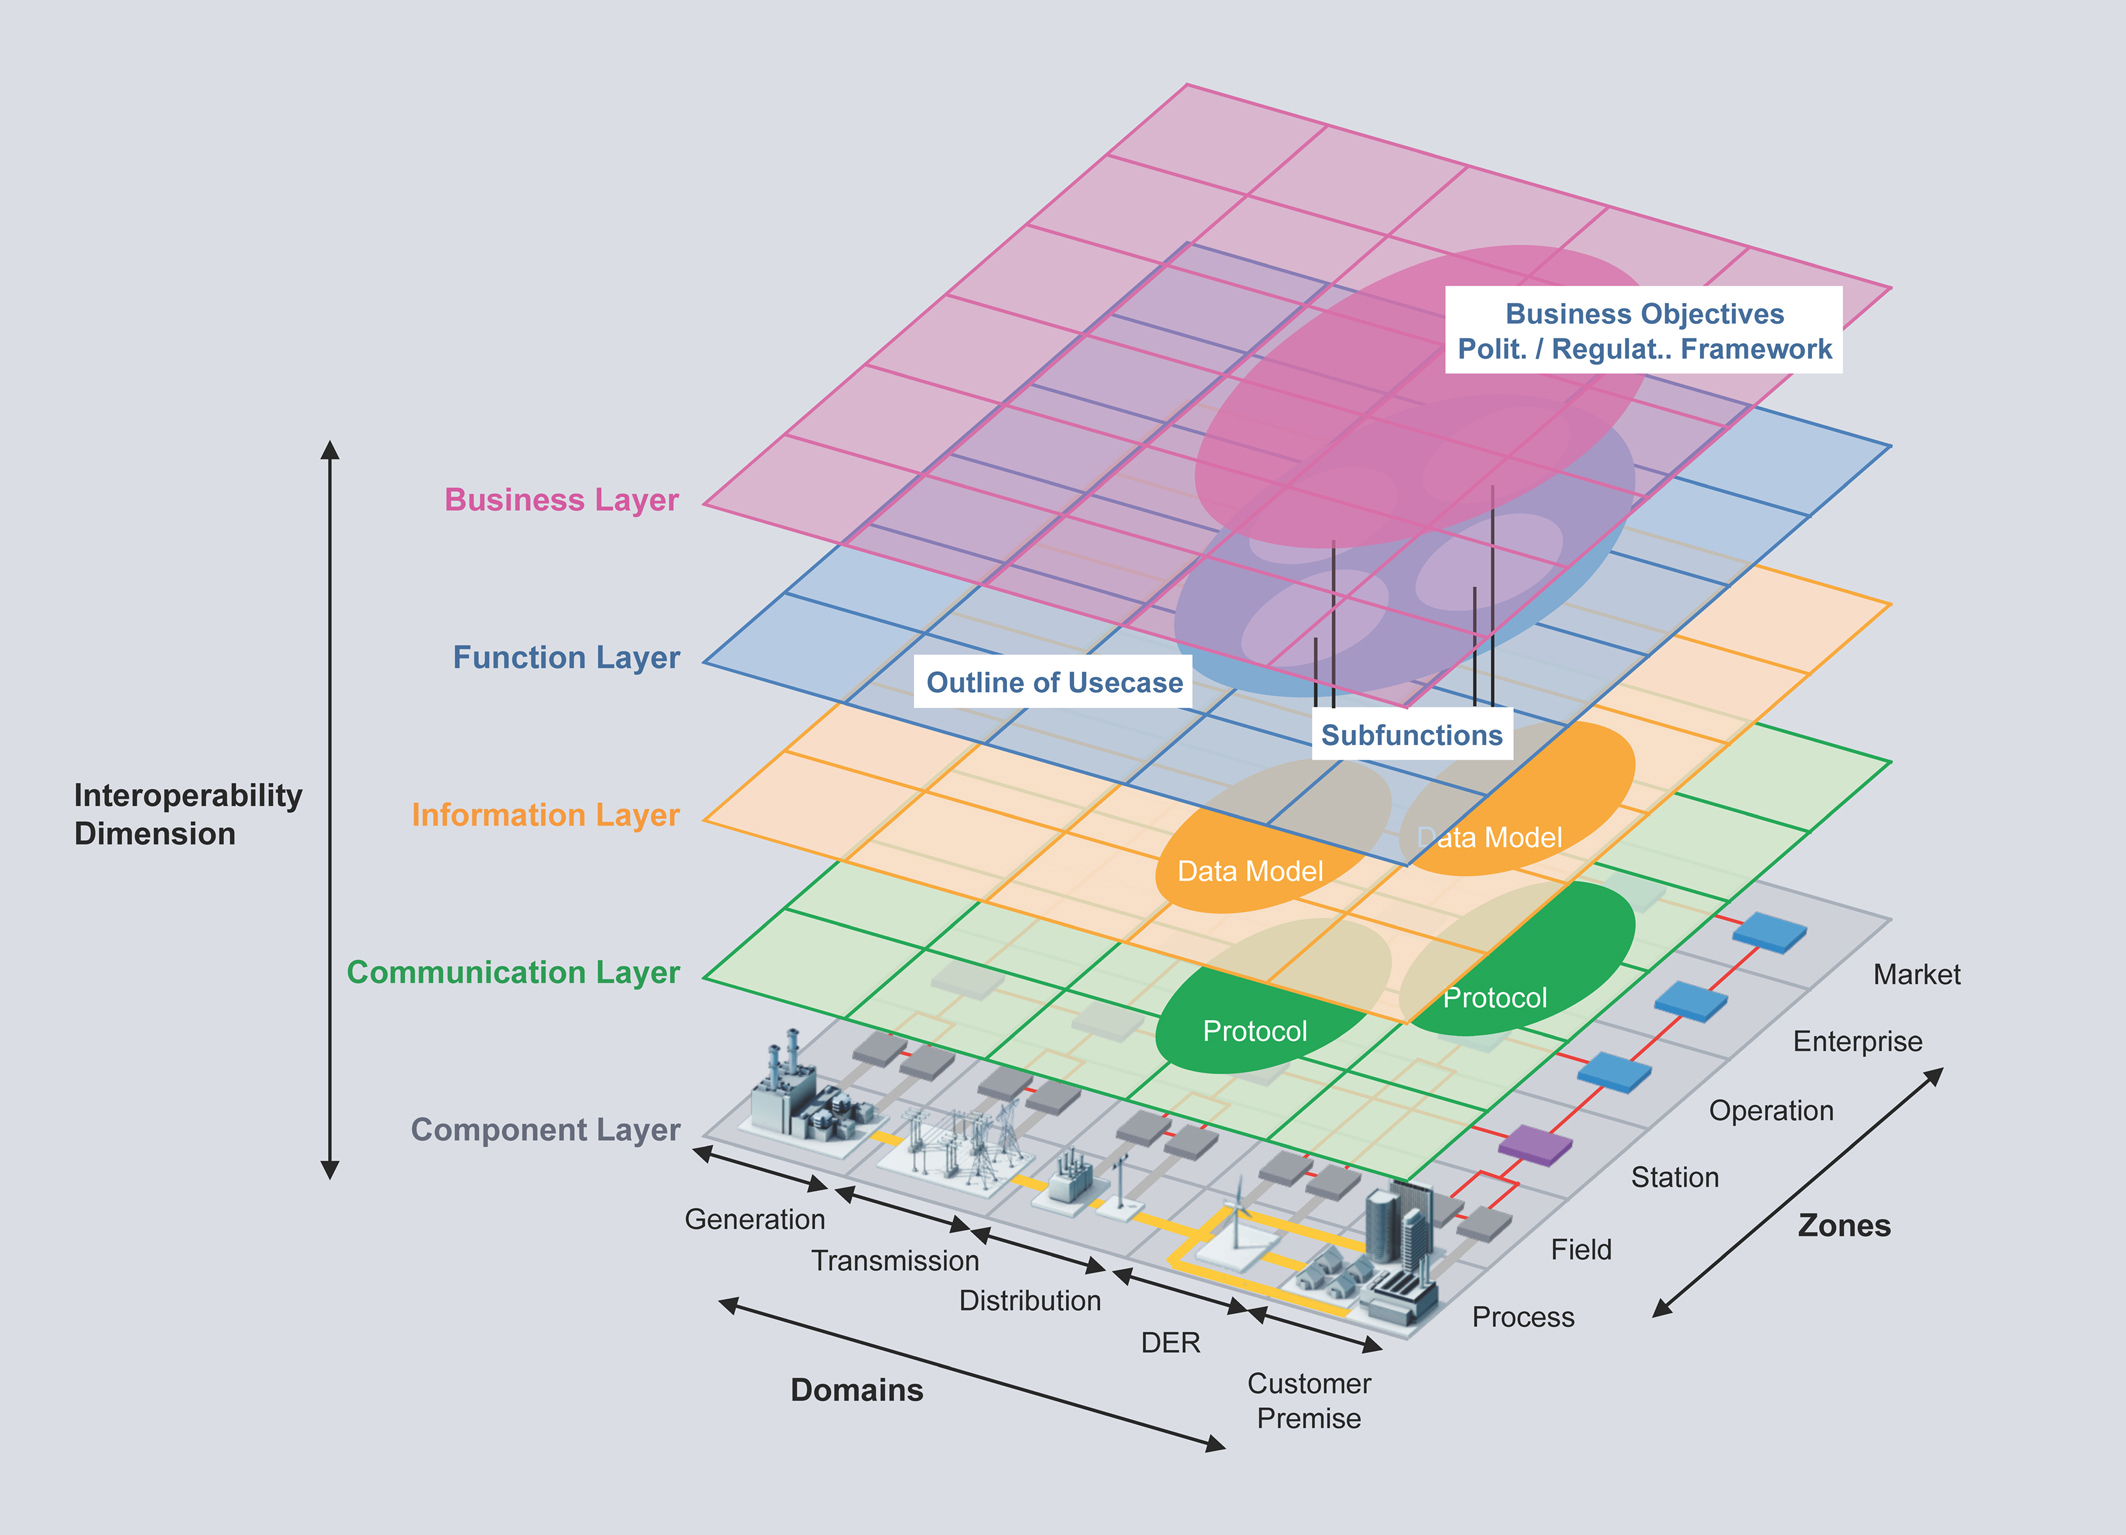
\includegraphics[scale=0.18]{Figures/SGAM_model}
	\caption{Smart Grid Architecture Model (SGAM) general overview}
	\label{fig:SGAM}
	
\end{figure}

\chapter{Electric Vehicle Charging Demand}
\label{ch:EV}
The aim of this chapter is to expose the probabilistic Plug-in electric vehicle (EV) charging model and to apply it in a distribution grid to evaluate the EV impact. The model is based on agent-based techniques, has probabilistic variables, includes queuing theory, and applies Monte Carlo methodology. The EV user's charging needs can be divided in two categories: private charging points and public charging points. Regarding private charging points, the EV charging demand depends strongly on private user's mobility needs and it includes variables as number of trips per day, driving distance, and arrival time. Also, the user's profile can be modelled with probabilistic variables as the EV model and the charging connection point. All these variables can be modelled with probabilistic distributions functions to obtain a probabilistic model with data from different sources. Additionally, public charging points are made available for EV users that need to plug-in the vehicle between trips to extend the vehicle autonomy. After that, the model is applied to a case study to analyze the impact to the power network. Probabilistic grid impact includes the probability to exceed a maximum voltage drop, and transformer and current saturations. The main impact is on saturations of lines and they can be reduced controlling private points but it does not make sense to control the public points.

\section{Introduction}

Electric vehicles (EVs) are presented as an alternative to current internal combustion vehicles powered by fossil fuels. Increasing oil prices, greenhouse gas emissions and environmental concerns of citizens boost interest in this technology. Energy supply from power networks is required and the impact on the distribution grids in a massive EV integration scenario has to be analysed in detail \cite{MIT_Grid}. Thus, studies about EV impact on power networks are needed to ensure the viability of the systems \cite{Clement2010,Sikai2010,EPE_Surtidor}.

The EV charging demand model should allow the analysis of possible effects of this new demand supplied in present-day power networks.

In order to do so, an EV charging model should include specific characteristics for each case, such as mobility, and it should allow one to compare different cases. Moreover, it should consider probability distribution functions (PDF) to analyse the uncertainties of possible EV charges. %justificacion probabilitat
In addition, this model should be designed to analyse the application of control strategies and enable their comparison.

%-----------------------------------------------State of the art
Literature proposes models to calculate the demand with respect to vehicle, charging infrastructure, mobility, and social parameters. \cite{Watts-Transp,Soares2012,Acha79,Valsera2012,Soares2011} use different parameters such as EV model, distance, and charging process among others to determine the EV charging demand.



\subsection{Contribution} \label{sec:contribution}

The state-of-the-art analysis defined seven subjects to be determined in the EV charging demand problem formulation:
\begin{itemize}
	\item EV type and model: the majority of current models simplifies this aspect with one model or an averaged model to represent a group of models. 
	\item Battery and the corresponding charging process: according to the literature review, the main difference found in literature is the charging process. The most common simplification is to consider a constant power but the appropriate way is to consider the relation between the SoC and the power consumed.
	\item Power infrastructure: the majority of articles consider the AC slow charging and the current limit depends in function on the country analysed.
	\item Mobility: the papers which consider it try to use the public data according to the country analysed.
	\item Social: the majority of the papers do not consider any economic or social variables.
	\item Simulation technique: the majority of papers take a bottom-down deterministic approach.
	\item How to analyse the impact on the power system: the majority of EV charging models avoid this issue and some of them try to optimise the EV charges to reduce some negative consequences.
\end{itemize}


The objective of this paper is to define a methodology based on agents to determine EV charging demand. The main contribution of this paper is to propose a methodology based on open data and combining social, technical and economic variables to calculate the EV charging demand and then determine the effects on the distribution networks. To do so, the parameters in literature were used separately; however, this paper proposes that all of them be combined in a single model in order to obtain more precise and realistic results. Figure \ref{fig:1st_scheme} shows the relation among the variables that are implemented in the present model. For example, EV agents have a set of constant parameters as EV model (technical), place of residence (social), GDP (economic) and others, as well as variable parameters of mobility such as distance, day of the week and others.

\begin{figure}[htbp]
	\centering
	\includegraphics[width=0.65\textwidth]{figures/EV_charging_demand/model_discussion}
	\caption{Basic scheme of EV charging demand parameters.}
	\label{fig:1st_scheme}
\end{figure}

%This paper proposes designing an EV charging demand model to take into account all these parameters and the relation between them. 
Finally, the result of this methodology leads to the charging process model for each EV agent, the total EV charging demand and consequently, it allows the impact on power networks to be analysed. The methodology proposed uses all sources from public data and it is applied using statistics from the city of Barcelona.

The EV charging demand model is defined as the electric demand from EVs during a certain time period, such as a day or week, to supply their batteries. EV charging demand depends on EV user driving needs and it is linked to EV characteristics and mobility of users.

%ABMS explanation:
The methodology proposed in this paper is the Agent-Based Modelling and Simulation (ABMS). The main strengths and applications of ABMS are listed as follows:

\begin{itemize}
	\item Heterogeneous individual components: EV model and mobility pattern of each EV owner.
	\item Flexible systems: to manage the charging demand of each EV.
	\item Influence of location: to consider the effects of the charging point location in the power network.
	\item Representation of social interactions: different types of EV owners could have different influences on the total system.
\end{itemize}

For these reasons, this methodology has been used for obtaining EV mobility patterns with an heuristic approach \cite{ElBanhawyABMS2012}. Furthermore, this methodology enables to simulate complex systems; for instance, load demand in power systems \cite{Acha79} or virtual power plants to include different types of agents \cite{vale2011vpp}. Thus, agent-based modelling has been selected for this research.

In this work, the EVs are a set of agents that has been defined as autonomous entities with their attributes and their processes are dynamic and time-dependent \cite{Macal,Bonabeau_AB}. It allows defining each EV driver as an agent considering the usage of each vehicle. Each agent is simulated individually including possible interactions through the relationships between agents. Section \ref{sec:Model} describes the characteristics of the agent-based model to obtain the charging demand from EVs and their impact on the distribution network.


\section{EV charging demand model}\label{sec:Model}

%Based on the scheme shown in Figure \ref{fig:1st_scheme} and following the ABMS methodology, 
According to the Figure \ref{fig:1st_scheme}, the parameters needed to model the EV charging demand can be clustered in three groups: the EV agent (section \ref{sec:EV_agent}), mobility pattern (section \ref{sec:Mob_pattern}) and the charging process (section \ref{sec:Charging_process}). All these parameters permit the determination of all charging processes needed to reach each destination.

\subsection{EV agent} \label{sec:EV_agent}

In the model developed, every EV agent represents an EV driver and its vehicle. The EV agent attributes are the EV model, the mobility needs, and the charging preferences.

The EV agent behaviours are the trips taken (mobility), their corresponding energy consumption from their battery, the energy consumed from the electricity network to charge the battery, and the charging decision. For instance, when EV agents reach their destination, their charging process begin depending on the EV agent preferences and the energy price.
The EV agent states with their corresponding variables are: waiting, driving, and charging.

%Retailer and aggregator
Moreover, there are two other agents that influence on EV agents behaviour: the Electricity Retailer Agent, who determines the electricity price for each instant, and the EV Aggregator Agent, who control the EV charges to reduce the electricity price. In the scenarios A, B and C, explained in the section \ref{sec:Case_study}, there is no EV aggregator and the price is determined by the Electricity Retailer Agent. In contrast, in the scenario D, also explained in section \ref{sec:Case_study}, the price is determined by the EV Aggregator Agent and the Electricity Retailer Agent does not influence on EV agents.

The main rule is that each EV agent, after each trip, takes the decision of charging in function of the battery state-of-charge, the electricity price and, in scenario D, the signal from the EV aggregator. Moreover, before changing the state of an EV agent from waiting to driving state, it is necessary that the battery has enough energy to reach the destination. The EV agents structure, their relationships with other agents and their environment are shown in Figure \ref{fig:EV_agent_structure}. Note that there are two environments related to the EV agents: spatial distribution and electricity network. Furthermore, the electricity market is the environment of Electricity Retailer Agent and EV Aggregator Agent.

When the simulation begins, the system computes the EV agent mobility needs and the battery state-of-charge variation.

\begin{figure}[h!]
	\centering
	\includegraphics[width=0.65\textwidth]{figures/EV_charging_demand/EV_agent}
	\caption{EV agent structure}
	\label{fig:EV_agent_structure}
\end{figure}

The first step to define the EV agents is the definition of EV agent groups ($C_{i}$) and their variables. For each group, it is necessary to define the number of agents (N), spatial distribution of influence and charging preferences.
And the EV model of each agent is defined with variables $EC_{i}$, $Aut_{i}$, $Cap_{i}$, $Ps_{i}$ and $Type_{i}$. The place of residence, defined in $R_{i}$, is considered for each agent, and this depends on the power network scenario and is modelled as a constant probability, based on public data such as \cite{Estad_BCN}. $R_{i}$ is linked with the charging point in home usage.

The PDF of each EV model is based on \cite{EV_Forecast_FandS} data and it just considers passenger vehicles and $Type_{i}$. This data was filtered for the case study in relation to EV model characteristics and technical data available from automakers. It is shown in Figure \ref{fig:EV_distrib}.

\begin{figure}[h!]
	\centering
	\includegraphics[width=0.65\textwidth]{figures/EV_charging_demand/EV_model_distribution}
	\caption{EV model probability distribution function $EV_{i}$. Based on \cite{EV_Forecast_FandS} and adapted to Barcelona-Spain and automakers data.}
	\label{fig:EV_distrib}
\end{figure}

In this model it is assumed that the PHEV drive is fully electric until the end of the energy stored in the battery, when they consume gasoline as hybrid electric vehicles. Other assumptions are exhibited in section \ref{sec:MonteCarlo}. 

\subsection{Mobility pattern} \label{sec:Mob_pattern}

Mobility variables are assigned to each EV agent in order to model its mobility behaviour. Different mobility patterns are based on open data sources. The variables considered to define a mobility pattern are defined as follows:

\begin{itemize}
	\item \textbf{Trips per day ($S_{i}$)}. The total trips are determined using a probabilistic variable which is generated through a Poisson distribution function, which is defined as \cite{xu2010GPS_Poisson} proposes with Poisson parameter ($\lambda$) of equation \ref{eq:Poisson}.
	
	\begin{equation} \label{eq:Poisson}
	P(k,\lambda)=(e^{-\lambda}\lambda^{k})/k!
	\end{equation}
	
	This parameter is based on the average statistic value. It should ensure at least two trips per day and is defined by \ref{eq:Lambda}.
	
	\begin{equation} \label{eq:Lambda}
	S_{i}=2+\lambda
	\end{equation}
	
	In the present study analysed, $\bar{S_{i}}=3.53$ trips/day are based on \cite{EMQ2006}.
	
	\item \textbf{Distance ($L_{i}$)} and \textbf{Distance per trip ($l_{ij}$)}. They are calculated using the exponential distribution function from public reports. Figure \ref{fig:Li} shows cumulative exponential distribution functions of distance travelled per day from different countries and the relation between $L_{i}$ and $l_{ij}$ is shown the following equation:
	\begin{equation} \label{eq:Li}
	L_{i}=\sum_{j=1}^{S_{i}} l_{ij}
	\end{equation}
	In the case study analysed, $\bar{L_{i}}=83$ km/day is based on \cite{Cetelem_Distancia}.
	If $l_{ij}>10$ km, the trip $j$ is considered as metropolitan considering Barcelona characteristics.
	
	\item \textbf{Destination ($D_{ij}$)}. 
	The model considers the reason of displacement to determine the destination.
	The reasons considered for the case study are based on the destination of each trip: for personal issues and for commuting.  It is strongly linked to grid node, where the EV is connected in relation to social data and mobility pattern. Destination is modelled with a constant PDF according to the power network topology.
	
	\item \textbf{Day of the week ($d_{i}$)} and \textbf{Time distribution ($m_{ij}$)}. These parameters allow knowing when an EV consumes energy as a function of the EV user's motivation to travel on a specific day. It is implemented in a PDF, as shown in Figure \ref{fig:mij} and Table \ref{tab:mij} as an example applied in the case study.
	
	\item \textbf{Velocity ($v_{ij}$)}. According to mobility data, velocity is modelled as a constant value, depending if the trip is urban or metropolitan. The average velocity from \cite{EMQ2006} and $v^{urban}=22.2$ km/h and $v^{metrop}=59.3$ km/h are applied.
	
	\item \textbf{Initial/Final time ($t_{0}$, $t_{1}$)}. The relation between them is the average velocity ($v_{ij}$) and distance ($l_{ij}$). Each pair of time variables is grouped in the matrix $Y_{i}$, which stores the mobility data of an EV agent.
	\begin{equation*} 
	Y_{i}=
	\begin{bmatrix}
	t_{0}^{1} & t_{1}^{1} \\
	\vdots & \vdots \\
	t_{0}^{S_{i}} & t_{1}^{S_{i}}
	\end{bmatrix}
	\quad
	\end{equation*}
	
	\item \textbf{Social variables}. Regarding the case study, it is necessary to take into account different variables such as Gross Domestic Product (GDP) and population density to determine the total number of agents (N) that could charge the EV at the same connection point. $C_{i}$ definition was described in section \ref{sec:EV_agent} and applied in section \ref{network}.
\end{itemize}

\begin{table}[htbp]
	\centering
	\caption{Time distribution considered in case study}
	\label{tab:mij}
	\begin{tabular}{ll}
		{\bf $m_{ij}$} & {\bf Description} \\
		\hline
		1 & Personal \\
		
		2 & Personal - Back home   \\
		
		3 & Professional \\
		
		4 & Professional - Back home \\
		\hline
	\end{tabular}  
\end{table}

\begin{figure}[h!]
	\centering
	\includegraphics[width=0.65\textwidth]{figures/EV_charging_demand/Prob_distance_day} 
	\caption{Probability distribution function of Distance $L_{i}$. \cite{Cetelem_Distancia}
		\label{fig:Li}}
\end{figure}

\begin{figure}[h!]
	\centering
	\includegraphics[width=0.65\textwidth]{figures/EV_charging_demand/time_distribution} 
	\caption{Probability distribution function of Time distribution $m_{ij}$. \cite{Cetelem_Distancia} \label{fig:mij}}
\end{figure}

\subsection{Charging process} \label{sec:Charging_process}

The charging process considered is slow charging - AC single-phase, depending on EV model, battery capacity, SoC, Energy required to arrive to next destination and time between displacements.

All the EV models are supposed to have Li-ion batteries and the slow charging process corresponds to a typical charging curve with two periods: constant period I and descendent period II \cite{Marra_baterias}. The power rate $Ps_{i}$ considered for charging is 3.7 kW (230 V, 16 A) because it is commonly available in residential and commercial areas in Europe \cite{Valsera2009} and it is also used by Marra et al. \cite{Marra_baterias}. The charging process depends on initial SoC and energy required ($E_{req}$) in the process. Figure \ref{fig:SC_profile} shows the charging process of a battery with $Cap_{i}$ and $E_{req}$ of 16.5 kWh.

In this model, it is assumed that period I requires 50$\%$ of time for a full charge and period II finishes when the power output reaches 8$\%$ of $Ps_{i}$.

\begin{itemize}
	\item Total energy (Battery capacity) is:  $Cap=E_{I} + E_{II}$.
	\item $\mu$ and $k$ are the exponential function parameters used in equation \ref{eq:expon}.
	\item Total process efficiency considered is 90$\%$ \cite{Clement2010}.
\end{itemize}

The equations of EV charging process described before are:
\begin{itemize}
	\item Period I is described by the following equations:
	\begin{equation} \label{eq:PI}
	P_{I}(t)=Ps_{i}
	\end{equation}
	\begin{equation} \label{eq:EI}
	E_{I}(t)=\int_{0}^{a} Ps_{i} dt
	\end{equation}
	\item Period II is described by the following equations:
	\begin{equation} 
	P_{II}(t) = k e^{-\mu t} \label{eq:expon}
	\end{equation}
	\begin{equation}
	E_{II}(t)=\int_{a}^{b} k e^{-\mu t}  dt
	\end{equation}
	where:
	\begin{equation} 
	\mu={-ln(0.08) \over a} \label{eq:mu}
	\end{equation}
	\begin{equation}
	k={Ps_{i} \over 0.08} \label{eq:k}
	\end{equation}
	\begin{equation}
	c=0.08 Ps_{i}
	\end{equation}
\end{itemize}

The initial SoC depends on the EV agent consumption. In the first simulation, the battery starts fully charged.

\begin{figure}[htbp]
	\centering
	\includegraphics[width=0.65\textwidth]{figures/EV_charging_demand/CL_charging_profile} 
	\caption{Slow charging profile - General scheme in relation to battery capacity. Based on \cite{Marra_baterias}
		\label{fig:SC_profile}}
\end{figure}

\subsection{Monte Carlo simulation} \label{sec:MonteCarlo}

This paper proposes using the algorithm shown in Figure \ref{fig:ev_abm_scheme_alg} to calculate the EV charging demand in a certain power network. This algorithm is based on Monte Carlo Methodology to include stochastic variables per agent and they are: $R_{i}$, $S_{i}$, $L_{i}$, $l_{ij}$, $D_{i}$, $t_{0}$, $t_{1}$ and $EV_{i}$. For this reason, it is necessary to define the number of iterations (T). Furthermore, to start the algorithm, it is necessary to define the number of agents (N) that charge the EV in the network analysed. The time step used is 5 minutes.

The algorithm is used to define the EV agent group, the mobility variables and then the charging process for each EV agent. 

\begin{figure}[h!]
	\centering
	\includegraphics[width=0.65\textwidth]{figures/EV_charging_demand/model_scheme_algorithm} 
	\caption{EV charging demand algorithm based on Monte Carlo. 
		\label{fig:ev_abm_scheme_alg}}
\end{figure}

\section{Case study}
\label{sec:Case_study}

The proposed EV charging demand model is applied in a case study with a 37-node IEEE test feeder adapted to a typical distribution network and mobility data of Barcelona (Spain) \cite{EMQ2006}. The modelling of the case study was implemented in Matlab $\copyright$ and the power flow is solved by means of the Newton-Raphson method.

Four charging scenarios (A-D) were defined to model EV agent behaviour, which are described in the following sections. The results are the energy ($Z_{i}$) and charging demand from EVs ($P(t,x)$) and the voltage profile in the distribution network.

\subsection{Distribution network} \label{network}

This case study is an adapted MV network 37-node IEEE test feeder, which is seen in Figure \ref{fig:37nodes}, and it applies Barcelona's mobility data. This network is adapted to a typical 25 kV MV network of Barcelona and the number of houses connected at the same MV/LV transformer \cite{Valsera2012}. In order to do that, it is necessary to consider social variables such as population density and technical regulation \cite{ITC-BT-10}. 
The maximum voltage drop permitted by the distribution system operator is 10$\%$ according to the EN 50160.

The total number of agents of group $C_{i}$ is defined in relation to network topology and population density of different neighbourhoods. According to social data from Barcelona and network branches, there are three zones: high, medium and low inhabitants per house and vehicles per inhabitant density. The farthest branch is linked with the high density zone. In this way, $D_{ij}$ of group $C_{1}$ at the end of the day is the corresponding network node.
In Barcelona, 38$\%$ of vehicles are driven each day and this percentage is used to determine active vehicles \cite{EMQ2006}.

\begin{figure}[htbp]
	\centering
	\includegraphics[width=0.65\textwidth]{figures/EV_charging_demand/Test-feeder_IEEE_37_nodes}
	\caption{MV network - IEEE Test-feeder 37 node.}
	\label{fig:37nodes}
\end{figure}

Table \ref{tab:connection_point} shows calculations to get N of group C1.

\begin{table*}[htbp]
	\centering
	\caption{Number of agents $ C_{1} $}
	\label{tab:connection_point}
	\begin{tabular}{rrrrrr}
		
		
		{\bf Zone} & {\bf Nodes}  & {\bf Inhab./}& {\bf Veh./} & {\bf Inhab.}  & {\bf Active} \\
		
		{\bf } & {\bf } & {\bf hou.} & {\bf Inhab.} &   {\bf } &      {\bf veh.} \\
		\hline
		High & 22-36 & 2.61& 0.50 & 5016 & 950 \\
		
		Medium & 3-5,6-15 & 2.52 & 0.47  & 2541 &  448 \\
		
		Low & 1,2,16-21 & 2.34 & 0.38 & 3288 &  471 \\
		\hline
		& &  & & \textbf{Total C1}& {\bf 1870} \\
		\hline
	\end{tabular}  
\end{table*}

\paragraph{\textbf{Load demand}}
Base load demand in this distribution network is based on system operator data \cite{ree} from national demand and it is adapted to network power capacity as 80$\%$ of HV/MV transformer power. Analysing the consumption in Spain between 2007 and 2011, load demand used in the case study is from 17 December 2007, when the maximum energy demand reached 45,911 MWh between 18:00 and 19:00. This allows analysing EV charging increase relative to this base load. 
%Change 14

The load presented in Figure \ref{fig:NoEV_demand} is the base case, without EVs, of the distribution system analysed. The peak demand is 10,640 kW and it occurs at 18:30. The load demand of the distribution system increases during the morning (8-10 o'clock), decreases during lunch time (13-16 o'clock) and increases during the evening (19-21 o'clock), when people come back home. The peak period is 79$\%$ higher than the valley period and the energy consumed during the course of a single day is 207.36 MWh. The voltage in the worst node is shown in Figure \ref{fig:NoEV_voltage}; the minimum voltage is 0.9707 p.u. at 18:30 and the maximum is 0.9839 p.u. at 4:45. The voltage follows a similar behaviour to the load demand. The lower limit of the voltage magnitude permitted by EN 50160 is 0.90 p.u.

%Change 13
\begin{figure}[htbp]
	\centering
	\subfigure[Load demand]{
		\label{fig:NoEV_demand}
		\includegraphics[width=0.4\textwidth]{figures/EV_charging_demand/NoEV/Residential_load_demand}}
	\subfigure[Voltage drop]{
		\label{fig:NoEV_voltage}
		\includegraphics[width=0.4\textwidth]{figures/EV_charging_demand/NoEV/voltage_residential_demand}}
	\caption{Residential and commercial demand without EVs}
\end{figure}


\subsection{Agent profile} \label{sec:agent_profile}

Six agent groups (C1 - C6) were defined to consider mobility and residence. Mobility is divided between personal and professional reasons. According to the usual place where the EV is connected at the end of the day, 3 different areas of residence were defined: local, urban and metropolitan. Local area refers to the distribution network analysed, urban refers to the city, and metropolitan is outside the city. Urban and metropolitan agents can plug in between displacements. On the other hand, local agents can charge at any time. Table \ref{tab:CS_users} shows the main characteristics of each group. N is the number of EVs of each agent that charge their batteries in the case study network.

\begin{table*} 
	\centering
	\caption{EV charging social characteristics in function of group} \label{tab:CS_users}
	\begin{tabular}{rrrrrr}
		
		{\bf $C_{i}$ } & {\bf $m_{ij}$ } & {\bf Active veh.} & {\bf N} &{\bf Area} & {\bf Preferences} \\
		\hline
		C1 &    1$\&$2 & 1870 & 561 & Local &   At-the-end \\
		
		C2 &    1$\&$2 & 449 & 135 & Urban & Between disp. \\
		
		C3 &    1$\&$2 & 273 & 82 & Metropolitan & Between disp. \\
		
		C4 & 3$\&$4 & 41 & 12 & Local &   At-the-end \\
		
		C5 & 3$\&$4 & 41 & 12 & Urban & Between disp. \\
		
		C6 & 3$\&$4 & 10 & 3 & Metropolitan & Between disp. \\
		\hline
		\textbf{Total} & & 2684 & 805 & & \\
		\hline
	\end{tabular}  
\end{table*}

Each group has specific energy requirements for charging ($E_{req}$). Preferences are related to when to charge and they are described above relative to agent group definition. Regarding the $E_{req}$ for each feasible charge between displacements, it is defined as the energy required to reach the next destination ($D_{ij}$) and distance ($l_{ij}$).

Mobility variables from Barcelona data \cite{EMQ2006} are implemented in the case study. $S_{i}$ depends on agent group, $d_{i}$ is the average weekday and $L_{i}$ is according to \cite{Cetelem_Distancia}.

\subsection{Charging scenarios}

According to agent preferences, $E_{req}$ and electricity market assumptions, four scenarios of EV charging demand are described, shown in Table \ref{tab:scen}.
\begin{table} [htbp]
	\centering
	\caption{Table of charging scenarios} \label{tab:scen}
	\begin{tabular}{lll}
		
		{\bf Charging} &  & {\bf Range} \\
		
		{\bf Scenario}& {\bf Description}      & {\bf anxiety} \\
		\hline
		A - Intensive charge & As soon as possible &       High \\
		
		B - Plug-and-Play & Just at home &        Medium \\
		
		C - Tariff controlled & Off-peak tariff &        Medium \\
		
		D - Smart charging & With Aggregator &        Low \\
		\hline
	\end{tabular}  
\end{table}

Scenarios A and B consider constant electricity price for the whole day. In scenario A, EVs charge at the end of each trip due to the high range anxiety of EV agents. In scenario B, the EV agents have lower range anxiety and they charge the vehicle at home, when SoC is lower than 20$\%$ or lower than $E_{req}$. In scenario C it is considered that the EV agents have a Time-of-Use (TOU) tariff, special for EVs \cite{kostkova2013introduction}. The cheapest period of this tariff begins at 1:00 am, based on the Spanish regulation \cite{RD_GestorCargas}, and then the EVs initiate the charge. The TOU tariff is an indirect control strategy to manage the EV charges. Scenario D considers one aggregator who manages all EV charges to consume the minimum power at the HV/MV transformer. This is based on an aggregator dedicated to reducing the impact in the transmission system, according to the Spanish regulation \cite{RD_GestorCargas}. This scenario shows a direct control strategy to manage the EV charges and the aggregator offers lower electricity prices for EV agents.
\subsection{Results}

The following discussion presents the results of the four scenarios simulated. The analysis is focused on the EV demand, total demand and the voltage drop in the worst node. Due to the probabilistic design of the model, the results are variable and the plots show the variation between the maximum and minimum energy consumption. Furthermore, the plots also show the average consumption as the most probable value.

All scenarios are simulated considering that 30$\%$ of active vehicles are electric (N), based on maximum scenarios in \cite{Clement2010,Putrus2009,MaitraCIRED2009}. $EV_{i}$ PDF is based on \cite{EV_Forecast_FandS}. What is also considered is that the EV agents with the value $L_{i}$ greater than 100 km are only PHEV ($Type_{i}$).

Impact on power system is analysed through voltage drop located in the farthest node, which is the 35. Figure \ref{fig:cdt-esc} shows the minimum voltage per node during the whole day and the maximum voltage drop is located in node 35.

\begin{figure}[htbp]
	\centering
	\includegraphics[width=0.65\textwidth]{figures/EV_charging_demand/voltage_profile/cdt_esc}
	\caption{Voltage per node.}
	\label{fig:cdt-esc}
\end{figure}

\paragraph{Iterations ($iter$)} 
The standard deviations (std. dev.) of power demand are evaluated to determine the number of iterations (T) to obtain valid results. To do that, a simulation with 1,200 iterations in scenario A for C1 group and with 30$\%$ of EVs was carried out.

Figure \ref{fig:std_iter} shows the std. dev. around hour 21 and it varies during the first 100 iterations significantly; it is nearly stable from iteration 200 and is constant from iteration 600. The ideal should be to do 600 iterations for all the cases, but the computing time to do it is very high and the volume of results to be stored requires a huge amount of memory. For these reasons, it is not possible to simulate 600 iterations for all the scenarios and the number of iterations has to be lower. The std. dev. varies around 10 kW from iteration 100 and from iteration 200, the results are more stable than previously. According to this, the number of iterations applied in the case study is 200. Other instances and scenarios are also checked and they comply with the std. dev. analysis. The consumption variation is also checked and it behaves similarly to the std. dev.

\begin{figure}[htbp]
	\centering
	\includegraphics[width=0.65\textwidth]{figures/EV_charging_demand/implementacionCL/STDeviation}
	\caption{Standard deviation variation in function of iterations T.}
	\label{fig:std_iter}
\end{figure}

\subsubsection{A - Intensive charge}

\paragraph{EV charging demand:}
As is shown in Figure \ref{fig:1-ScA}, the EV charging demand presents two peaks with more consumption around 10:00 and 19:00. Both peaks are related to Barcelona's mobility pattern illustrated in Figure \ref{fig:mij}, which shows the same peaks: the peak during the morning is caused by professional mobility and the peak during the evening is caused by professional and personal back home reasons. The EV charging demand variability, the difference between the minimum and the maximum case, is significant in this scenario, and it can reach the 50$\%$ of the EV consumption as it occurs at 20:00.

The EV peak demand is near to 500 kW and the total peak demand is 11.04 MW, 3.75$\%$ higher than in the base case without EVs, as Figure \ref{fig:tot-A} demonstrates. Furthermore, the peak during the morning is coupled with the residential and commercial demand. This is reflected in Figure \ref{fig:tot-A}, where the active power increase is steeper from 6 to 12 hours due to the EV charging demand.

\paragraph{Impact on power system:}
Figure \ref{fig:v-A} shows that the minimum voltage in node 35 is 0.9694 p.u. and it is 0.13$\%$ lower than in the No EV case, which is higher than the lower limit of the standard of 0.9 p.u. 
\begin{figure*}[htbp]
	\centering
	\subfigure[EV charging demand]{
		\label{fig:1-ScA}
		\includegraphics[width=0.30\textwidth]{figures/EV_charging_demand/EV_demand/EVDem_ScA_30EVv3}}
	\subfigure[Total demand]{
		\label{fig:tot-A}
		\includegraphics[width=0.3\textwidth]{figures/EV_charging_demand/Total_demand/TotalDem_ScA_30EVv3}}
	\subfigure[Voltage drop]{
		\label{fig:v-A}
		\includegraphics[width=0.3\textwidth]{figures/EV_charging_demand/voltage_profile/voltage_ScA_30EVv3}}
	\caption{A - Intensive charge}
\end{figure*}

\subsubsection{B - Plug-and-Play}

\paragraph{EV charging demand:}
In this scenario, the EV agents prefer to charge at home, according to the back home time distributions ($m_{ij}$). As shown in Figure \ref{fig:1-ScB}, the first peak demand is lower than in scenario A because the agents do not charge at work. Moreover, the second peak demand is higher than before because the agents have not charged at work and the energy required by them is higher than in scenario A. In this scenario, the EV charging demand variability is also significant and it can reach the 33$\%$ of the EV consumption, as it occurs at 20:00.

As Figure \ref{fig:tot-B} shows, this effect causes that the peak during the morning in the total demand is lower than the previous case. And the peak during the evening is higher due to the energy required and the maximum power consumed is 11,12 MW at 18:35 and the relative increase from the case without EV is 4.51$\%$. Moreover, the power consumption during the night is higher than in case A, because the SoC of EV agents when they arrive at home is lower than previously.

\paragraph{Impact on power system:}
Figure \ref{fig:v-B} shows that the combination of the peak from the residential demand with the EV demand causes a higher voltage drop than scenario A due to the different behaviours of the EV agents. The minimum voltage reached during the peak demand is 0.9691 p.u., 0.16$\%$ lower than the case without EV, and higher than the lower limit of 0.90 p.u.

\begin{figure*}[htbp]
	\centering
	\subfigure[EV charging demand]{
		\label{fig:1-ScB}
		\includegraphics[width=0.3\textwidth]{figures/EV_charging_demand/EV_demand/EVDem_ScB_30EVv3}}
	\subfigure[Total demand]{
		\label{fig:tot-B}
		\includegraphics[width=0.3\textwidth]{figures/EV_charging_demand/Total_demand/TotalDem_ScB_30EVv3}}
	\subfigure[Voltage drop]{
		\label{fig:v-B}
		\includegraphics[width=0.3\textwidth]{figures/EV_charging_demand/voltage_profile/voltage_ScB_30EVv3}}
	\caption{B - Plug-and-Play}
\end{figure*}

\subsubsection{C - Tariff controlled}

\paragraph{EV charging demand:}
In this case, the TOU tariff causes that the EV agents begin to charge at 1:00, when the energy is cheaper. Therefore, the EV charging demand presents a peak of 1.86 MW at this moment due to the simultaneous EV charges, as seen in Figure \ref{fig:1-ScC}. What is more, the control reduces the EV charging demand variability.

The consumption during the rest of the day is related to the energy required ($E_{req}$) to reach the next destination ($D_{ij}$) and the low SoC of each EV agent. The maximum power consumed is 10.8 MW at 18:30, which means an increase of 1.5$\%$ from the original case.

Figure \ref{fig:tot-C} shows that this EV peak happens during the off-peak period and the total demand increase is not significant. Despite this, the power generation gradient could be a problem, which should be analysed from the point of view of the power generation and from the system stability point of view.

\paragraph{Impact on power system:}
The minimum voltage, shown in Figure \ref{fig:v-C}, is similar to the original case without EVs. The minimum voltage reached is 0.9702 p.u., 0.05$\%$ lower than without EVs, and higher than 0.90 p.u. The voltage variation at 1:00 could be a problem, which could be analysed in a transient analysis.
\begin{figure}[htbp]
	\centering
	\subfigure[EV charging demand]{
		\label{fig:1-ScC}
		\includegraphics[width=0.3\textwidth]{figures/EV_charging_demand/EV_demand/EVDem_ScC_30EVv3}}
	\subfigure[Total demand]{
		\label{fig:tot-C}
		\includegraphics[width=0.3\textwidth]{figures/EV_charging_demand/Total_demand/TotalDem_ScC_30EVv3}}
	\subfigure[Voltage drop]{
		\label{fig:v-C}
		\includegraphics[width=0.3\textwidth]{figures/EV_charging_demand/voltage_profile/voltage_ScC_30EVv3}}
	\caption{C - Tariff controlled}
\end{figure}

\subsubsection{D - Smart charging}

\paragraph{EV charging demand:}
Figure \ref{fig:1-ScD} shows the EV charging demand controlled by the aggregator which controls domestic EV charges. The EV charging demand is shifted to the valley period to reduce the consumption through the HV/MV transformer and to minimise the impact on the transmission system. According to this, the EV charges occur between 2 and 8 o'clock and the variability, the difference between the minimum and the maximum case, is very small.

Figure \ref{fig:tot-D} shows that the total demand increases during the valley periods and the power consumption is constant at 6.6 MW. During the rest of the day, sporadic charges could occur, but the mean curve is near to the case without EVs.

\paragraph{Impact on power system:}
The minimum voltage is not increased by the EV charges, as is exhibited in Figure \ref{fig:v-D}. The voltage during the valley period is lower than in the original case according to the total demand, but this voltage is higher than during the peak hours, and the difference between the minimum voltages is 0.02$\%$, and the minimum value of 0.90 p.u. is not reached.

\begin{figure}[htbp]
	\centering
	\subfigure[EV charging demand]{
		\label{fig:1-ScD}
		\includegraphics[width=0.3\textwidth]{figures/EV_charging_demand/EV_demand/EVDem_ScD_30EVv3}}
	\subfigure[Total demand]{
		\label{fig:tot-D}
		\includegraphics[width=0.3\textwidth]{figures/EV_charging_demand/Total_demand/TotalDem_ScD_30EVv4}}
	\subfigure[Voltage drop]{
		\label{fig:v-D}
		\includegraphics[width=0.3\textwidth]{figures/EV_charging_demand/voltage_profile/voltage_ScD_30EVv3}}
	\caption{D - Smart charging}
\end{figure}

The summary of all the scenarios is presented in Table \ref{tab:max_result}. Voltage value is the minimum and it means the maximum voltage drop.

\begin{landscape}
	\begin{table*}[h!]
		\centering
		\caption{Maximum results}
		\label{tab:max_result}
		\begin{tabular}{lrrrrrrr}
			& {\bf EV demand} & {\bf Peak } & {\bf Total demand}& & {\bf Peak } & {\bf Voltage} & \\
			{\bf Scenario} & {\bf (Max) [kW]} & {\bf Time} & {\bf (Max) [kW]} & {\bf Variation} & {\bf Time} & {\bf (Min)  [p.u.]} & {\bf Variation}  \\
			\hline
			No EV &  & 18:30& 10640 & & 18:30 & 0.9707 &    \\
			A - Intensive charge & 457 & 18:30 & 11040 & 3.76$\%$ & 18:30 & 0.9694 & -0.13$\%$  \\
			B - Plug-and-Play & 628 & 18:35 & 11120 & 4.51$\%$ & 18:35 & 0.9691 & -0.16$\%$  \\
			C - Tariff controlled & 1857 & 01:00 & 10800&  1.50$\%$ & 18.30 & 0.9702 & -0.05$\%$  \\
			D - Smart charging & 799 & 04:30 & 10720 & 0.75$\%$ & 18:35 & 0.9705 & -0.02$\%$  \\
			\hline
		\end{tabular}
	\end{table*}
\end{landscape}


Box plots \ref{fig:boxplotA}, \ref{fig:boxplotB}, \ref{fig:boxplotC} and \ref{fig:boxplotD} show total consumption in each node and this is compared to MV/LV transformer capacity. The results show that the nodes with less capacity could reach the nominal value in some cases, but the average value is under nominal power. In the case of scenario D, total demand never exceeds the nominal capacity of transformers, which means that there is enough capacity to supply the EVs.

\begin{figure*}[htbp]
	\centering
	\subfigure[A - Intensive charge]{
		\label{fig:boxplotA}
		\includegraphics[width=0.45\textwidth]{figures/EV_charging_demand/boxplots/Boxplot_EscA_30EVv2}}
	\subfigure[B - Plug-and-Play]{
		\label{fig:boxplotB}
		\includegraphics[width=0.45\textwidth]{figures/EV_charging_demand/boxplots/Boxplot_EscB_30EVv2}}
	\subfigure[C - Tariff controlled]{
		\label{fig:boxplotC}
		\includegraphics[width=0.45\textwidth]{figures/EV_charging_demand/boxplots/Boxplot_EscC_30EVv2}}
	\subfigure[D - Smart charging]{
		\label{fig:boxplotD}
		\includegraphics[width=0.45\textwidth]{figures/EV_charging_demand/boxplots/Boxplot_EscD_30EVv2}}
	\caption{Total demand in each MV/LV transformer}
\end{figure*}

\section{Conclusions}

The probabilistic agent-based model (ABM) obtained in this paper allows the EV charging demand to be determined, taking into account different variables of EV characteristics such as battery capacity and energy consumption of each trip, economic and social attributes, mobility needs, and charging strategies of each agent. The model developed takes into account the interaction of these variables, allowing the obtainment of better accuracy in the results.

The probabilistic approach is useful to include the uncertainties related to the real behaviour of EV users, like the time distribution and energy consumed on each trip. Therefore, the model permits determining the impact provoked on the grid by these uncertainties.

Moreover, the model proposed is a benchmark to compare case studies, such as different cities or areas in the same city. Due to this model, the weak regions of the grid or the areas with high EV density can be detected.

The case study presented shows that the uncertainties cause variability in the EV charging demand in scenarios without control on the EVs, as it is shown in scenarios A and B. In contrast, the consumption variability in scenarios with indirect and direct control on the EV charges, like scenarios C and D, respectively, is small.

The distribution feeder analysed in the presented case study does not have a significant impact with the smart charging strategy (D) during the off-peak period and all EV agents can charge their EV. In contrast, some MV/LV transformers could exceed their nominal power in the scenarios without control. The voltage in all the scenarios is higher than the limit of 0.90 p.u. according to the EN 50160.

As further work, it could be very interesting to analyse the dynamic behaviour of the system in case C during the connection of all EV at 1:00. Furthermore, the model permits analysing the impact on distribution networks, but it can be applied for transmission and low voltage grids, too. Finally, this model could be applied and compared with a real distribution network with EVs to verify the accuracy of the model.

\chapter{Methodology - Design of a electricity micro-market}
The structure of this thesis is based on scientific methodology. The proposed structure consists on analysing the current integration of renewable energies in the electricity market and identifying a solution to improve the performance of the system.

\section{Local electricity micro-market proposal}

As it is said in section \ref{sec:SoA_mm}, the micro-market can be divided in two micro-markets: before and after the wholesale day-ahead market. 
The objective of the micro-market before the day-ahead, entitled as day-ahead micro-market, is to organize the resources and it could have a similar structure of the current day-ahead market.
In contrast, the micro-market after the day-head, entitled as micro-market for deviations, is to adjust the deviations with the minimum cost.

Regarding the micro-market before the day-ahead wholesale market, figure \ref{fig:micro-market} shows an example which exemplifies the case of a  of 11 kV meshed distribution grid with four nodes; two nodes with renewable generation and one with a combustion engine generation. The topology of the grid is meshed considering that there are remote controlled switchgears which permit to isolate faults.

The generation and consumption configuration is solved with the AC optimal power flow (OPF) implemented in MATPOWER, a toolbox designed by Ray Zimmerman \cite{MATPOOWER}. The OPF minimize the objective function which considers the generation costs. Moreover, MATPOWER has the Smart Market package which permits to include bids and offers in the OPF's objective function as new costs.

Moreover, the virtual market agent represents the energy that can be consumed or generated from the grid. The bids and offers of market agent correspond from a forecast of the wholesale day-ahead market.

Regarding the bids$\&$offers of each bus, the blue lines are the bids from the consumption side and the red lines are the offers from the generation side. All offers and bids are represented by each grid node and the micro-market auction is the sum of all buses. After the auction, the price applied to all consumers and producers is the same to avoid unfair situations due to network constraints.

The red arrows from the generators are the active flow direction. In the case of renewable generators they only produce active power because the solar inverters are programmed to produce as much active power as possible with a power factor near to 1.

Regarding the flows through the lines, red arrows represent the active power flow and the green ones represent the reactive power flow measured at the origin of the line. Due to the fact that the reactive power only comes from the grid, the line between nodes 2 to 3 reaches its maximum thermal limit of 5.53 MVA.

The advantages of the proposal of local electricity-markets are firstly the capability to include network constraints in the market. The result of the auction permits to obtain a feasible configuration instead of a solution only from the economic point of view. Secondly, local micro-markets operation could be independent from the wholesale market, hence they can better handle changing situations from EVs, DG generation, demand steps and storage. 

The result of the case presented is:
\begin{itemize}
	\item Energy matched: 21.84 MWh
	\item Price matched: 6 EUR/MWh
	\item Objective function: -505.57 EUR
\end{itemize}

\begin{landscape}
	\begin{figure}[h!]
		\centering
		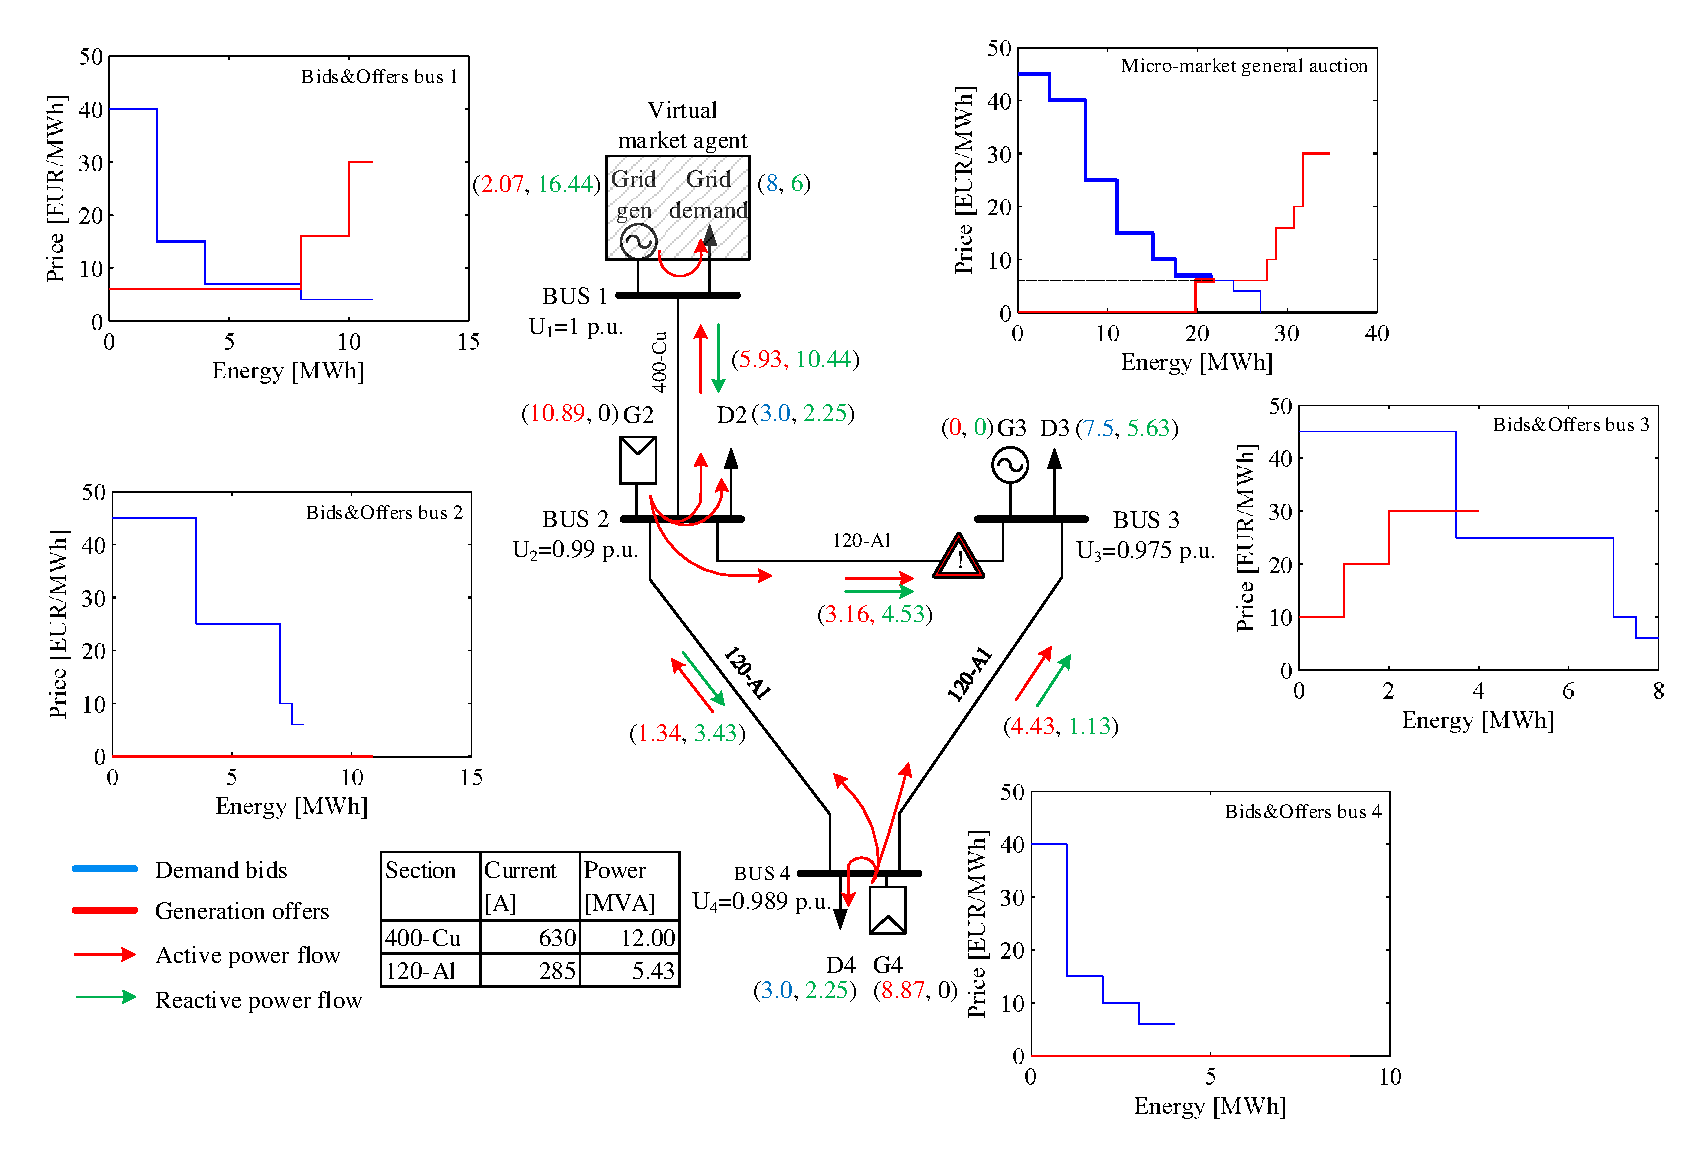
\includegraphics[scale=0.6]{Visios/Local_market_scheme}
		\caption{Local electricity micro-market with four nodes, two renewable generators, and the connection to the main grid with the virtual market agent}
		\label{fig:micro-market}
	\end{figure} 
\end{landscape}

Regarding the micro-market after the day-ahead wholesale market it is still pending to be developed but according to the initial investigations such as \cite{ampatzis2014}, this will based on continuous double-sided auction to incentives the flexibility of consumers and generators.  

\chapter{Working plan}
The different works, which correspond to the objectives of the thesis are detailed below and organized in the Gantt diagram of figure \ref{fig:Gantt}

\begin{enumerate}
	\item Study of the state of the art
	\item EV fleet charging model
	\subitem Modelling a EV battery charging profile
	\subitem Modelling a EV fleet
	\subitem Modelling the impact on a distribution network
	\item Market architecture
	\subitem Market use cases
	\subitem Architecture layers
	\item Modelling of storage in distribution grids
	\subitem Develop a battery model for market integration
	\subitem Implement the battery model in distribution grids
	\item Micro-market design
	\subitem Day-ahead micro-market design
	\subitem Micro-market for deviations design
	\item Micro-market implementation in laboratory platform
	\subitem Software programming
	\subitem Comparison between model and experimental results
\end{enumerate}

\begin{landscape}
	\begin{figure}[h!]
		\centering
		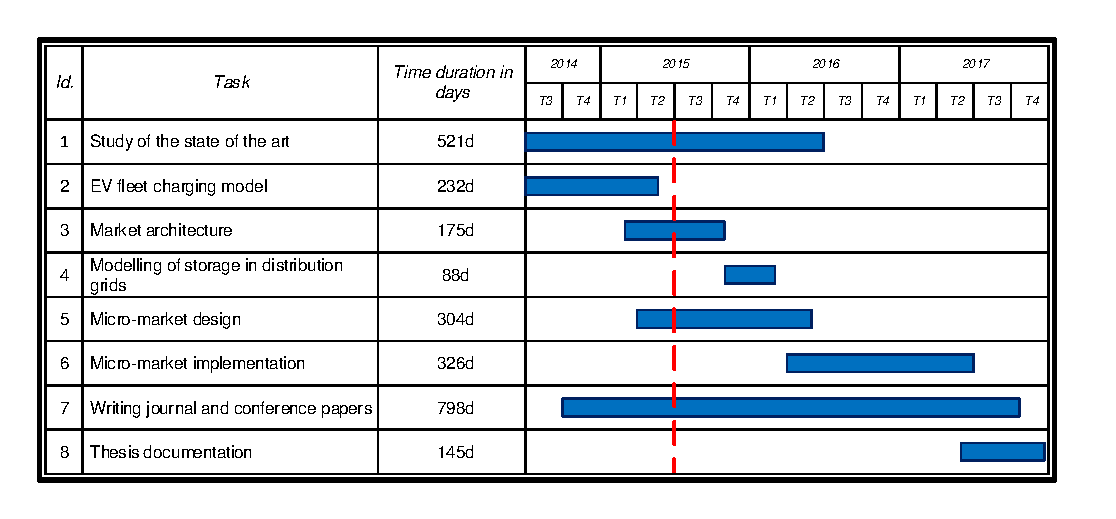
\includegraphics[scale=1]{Visios/Gantt}
		\caption{Gantt diagram of the PhD}
		\label{fig:Gantt}	
	\end{figure}
\end{landscape}


\chapter{Publications}
\label{cap:publicacions}
From the work detailed on previous chapters, several publications have resulted.

\section{Jourmal articles}
\begin{itemize}
	\item \textbf{Pol Olivella-Rosell}, Roberto Villafafila-Robles, Andreas Sumper, Joan Bergas Jan\'{e}. 
	''Probabilistic Agent-Based Model of Electric Vehicle Charging Demand to Analyse the Impact on Distribution Networks'' Energies 2015, 8(5), 4160-4187; doi:10.3390/en8054160.
	\item Niels Leemput, Frederik Geth, Juan Van Roy, \textbf{Pol Olivella-Rosell}, Johan Driesen and Andreas Sumper. 
	''MV and LV Residential Grid Impact of Combined Slow and Fast Charging of Electric Vehicles'' Energies 2015, 8(3), 1760-1783; doi:10.3390/en8031760.
	\item Eduardo Prieto-Araujo, \textbf{Pol Olivella-Rosell}, Marc Cheah-Ma\~{n}e, Roberto Villafafila-Robles,
	Oriol Gomis-Bellmunt.
	 ''Renewable energy emulation concepts for microgrids'' Renewable and Sustainable Energy Reviews 2015.
\end{itemize}

\section{Book chapter}
\begin{itemize}
\item Plug In Electric Vehicles in Smart Grids, Integration Techniques.
Edited by  Sumedha Rajakaruna, Farhad Shahnia, Arindam Ghosh. Springer.
Chapter: Impact Evaluation of Plug-in Electric Vehicles on Power System
\textbf{Pol Olivella-Rosell}, Roberto Villafafila-Robles, Andreas Sumper.
\end{itemize}

\section{Conference papers}
\begin{itemize}
\item Roberto Villafafila-Robles, Francesc Girbau-Llistuella, \textbf{Pol Olivella-Rosell}, Antoni Sudri\`{a}-Andreu, Joan Bergas-Jane.
''Assessment of impact of charging infrastructure for electric vehicles on distribution networks.''. 
Power Electronics and Applications (EPE), 2013 15th European Conference on. IEEE, Lille, France, September 2013.
\item Bernat Felisart-Serlavos, Roberto Villafafila-Robles, \textbf{Pol Olivella-Rosell}, Rodrigo Ramirez-Pisco, Antoni Sudri\`{a}-Andreu. ''Energy Market Regulations for Electric Vehicle Encourage. Study of Current Frames.''. XIII conferencia hispano-lusa de ingenier\'{\i}a el\'{e}ctrica (XIIICHLIE), Valencia, Spain, July 2013.
\item Maurici Yag\"{u}es, \textbf{Pol Olivella-Rosell}, Roberto Villafafila-Robles, Andreas Sumper. 
''Ageing of Electric Vehicle Battery considering Mobility Needs for Urban Areas.''. International Conference on Renewable Energies and Power Quality (ICREPQ'14), Cordoba, Spain, April 2014.
\item Victor Depoorter, \textbf{Pol Olivella-Rosell}, Antoni Sudri\`{a}-Andreu, Jordi Giral-Guardia, Andreas Sumper. 
''Simulation of a small-scale electricity generation system from biomass gasification.''. International Conference on Renewable Energies and Power Quality (ICREPQ'14), Cordoba, Spain, April 2014.
\item \textbf{Pol Olivella-Rosell}, Guillem Bosch-Llufriu, Roberto Villafafila-Robles, Daniel Heredero-Peris, Mario Kova\u{c}evi\'{c}, Niels Leemput. ''Assessment of the Impact of Electric Vehicles on Iberian Day-ahead Electricity Market''. IEEE International Electric Vehicle Conference 2014, Florence, Italy.
\item Dami\`{a} Valero-Bover, \textbf{Pol Olivella-Rosell}, Roberto Villafafila-Robles, Silvia Cestau-Cubero. ''Performance Analysis of an Electric Vehicle Fleet for Commercial Proposes''. IEEE International Electric Vehicle Conference 2014, Florence, Italy.
\item \textbf{Pol Olivella-Rosell}, Guillem Vi\~{n}als-Canal, Andreas Sumper, Roberto Villafafila-Robles, Bernt A. Bremdal, Iliana Ilieva. ''Day-ahead micro-market design for distributed energy resources''. IEEE International Energy Conference 2016, Leuven, Belgium.
\item Iliana Ilieva, Bernt A. Bremdal, Stig \O{}degaard Ottesen, Jayaprakash Rajasekharan, \textbf{Pol Olivella-Rosell}. ''Design characteristics of a Smart Grid Dominated Local Market''. CIRED Workshop 2016, Helsinki, Finland.
\end{itemize}

\section{Other publications}

\begin{itemize}
\item Jordi Giral-Guardia, Angel Llad\'{o}, \textbf{Pol Olivella-Rosell}, Antoni Sudri\`{a}-Andreu.
''La biomasa como fuente de energ\'{\i}a el\'{e}ctrica a peque\~{n}a escala.'' Enero 2013, Vol. 447, Autom\'{a}tica e Instrumentaci\'{o}n.
\item Roberto Villaf\'{a}fila-Robles,\textbf{ Pol Olivella-Rosell}, Antoni Sudri\`{a}-Andreu.
''El auge de los recursos energ\'{e}ticos distribuidos'' Enero 2013, Vol. 447, Autom\'{a}tica e Instrumentaci\'{o}n.
\item Roberto Villaf\'{a}fila-Robles, \textbf{Pol Olivella-Rosell}, Antoni Sudri\`{a}-Andreu.
''El ecosistema del veh\'{\i}culo el\'{e}ctrico'' Junio 2013, Vol. 452, Autom\'{a}tica e Instrumentaci\'{o}n.
\end{itemize}

	\bibliographystyle{unsrt}
	\bibliography{references}
	\addcontentsline{toc}{chapter}{References}
\end{document}

